\documentclass[a4paper,12pt]{article}
\usepackage[utf8]{inputenc}

\usepackage{amsmath}
\usepackage{graphicx}
\usepackage{float}
\usepackage[font=small,labelfont=bf]{caption}
\usepackage{subcaption}
\usepackage{wrapfig}
\usepackage{booktabs}
\usepackage{multicol}
\usepackage{longtable}
\newcommand{\tabitem}{~~\llap{\textbullet}~~}
\usepackage{xcolor}
\definecolor{commentgreen}{RGB}{2,112,10}
\definecolor{eminence}{RGB}{108,48,130}
\definecolor{weborange}{RGB}{255,165,0}
\definecolor{frenchplum}{RGB}{129,20,83}
\usepackage{listings}
\lstset{
	basicstyle=\small,
	columns=fullflexible,
	breaklines=true,
	postbreak=\mbox{\textcolor{red}{$\hookrightarrow$}\space},
	frame=tb,
	%frame=single
	tabsize=2,
	showstringspaces=false,
	numbers=left,
	%upquote=true,
	commentstyle=\color{commentgreen},
	keywordstyle=\color{eminence},
	stringstyle=\color{red},
	emph={int,char,double,float,unsigned,void,bool,var},
	emphstyle={\color{blue}},
	escapechar=\&,
	% keyword highlighting
	classoffset=1, % starting new class
	otherkeywords={>,<,.,;,-,!,=,~},
	morekeywords={>,<,.,;,-,!,=,~},
	keywordstyle=\color{weborange},
	classoffset=0
}
\usepackage{suffix}
\newcommand\sectionauthor[1]{\authortoc{#1}}
\usepackage{hyperref}
\hypersetup{
	citecolor=blue,
	colorlinks=true, %set true if you want colored links
	linktoc=all,     %set to all if you want both sections and subsections linked
	linkcolor=blue,  %choose some color if you want links to stand out
}

\usepackage[
	backend=biber,
	style=alphabetic,
	citestyle=alphabetic
]{biblatex}
\addbibresource{main.bib}

\newcommand{\authortoc}[1]{%
  \addtocontents{toc}{\vskip-5pt}%
  \addtocontents{toc}{%
    \protect\contentsline{subsection}%
    {\hskip2.3em\mdseries\scshape\protect\scriptsize#1}{}{}}
  \addtocontents{toc}{\vskip5pt}%
}

\usepackage[left=2.5cm,right=2.5cm,top=3cm,bindingoffset=0mm]{geometry}
\usepackage{csquotes}
\linespread{1.3}

\begin{document}
	\pagenumbering{gobble}
\setlength\parindent{0pt}
\begin{titlepage}
	\centering
	\vspace{5cm}
	{\scshape\LARGE Greenhouse yield prediction \par}
	\vspace{0.5cm}
	{\scshape Systems Engineering Meets Life Sciences \par}
	{\scshape Project report\par}
	\vspace{2cm}
	{\large Authors\par}
	\vspace{0.5cm}
	\input{authors}

	\vfill
	Advisor:\par
	Prof. Dr. Visvanathan  \textsc{Ramesh}
	\vfill
	\huge
	DRAFT
	\vfill

	% Bottom of the page
	{\large Prepared at Goethe University Frankfurt am Main \\ \today\par}
\end{titlepage}

\tableofcontents
\newpage
\pagenumbering{arabic}
\section{User-View}

Test
\graphicspath{{members/ssr/figures/}}

\subsection{Greenhouse}\label{subsec:greenhouse}

A greenhouse is a special building for the lone purpose of growing plans under optimal
conditions.
It‘s build of (semi)transparent walls and a roof - depending on the specific
needs of the crops and the location.
Environmental controls govern the atmosphere - ideally - for optimal growing conditions.
The controls typically regulate temperature, humidity, lighting, irrigation and the
nutrition provided through the soil etc.\\

\begin{figure}[H]
    \centering
    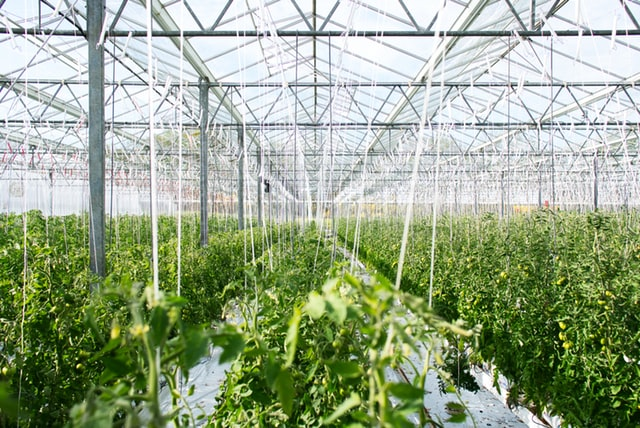
\includegraphics[width=0.8\textwidth]{user-view/greeenhouse_erwan_hesry_unsplash.jpg}
    \caption{Inside a greenhouse}
\end{figure}

Only crops with similar or same optimal growing conditions are grown within each greenhouse
since different crops have difference optimal growing conditions but typically only one crop
variety is grown within each greenhouse.\\

While the greenhouse system won't be introduced here further - since it's not the focus
of this project - it's nonetheless worthwhile to get a high-level picture of the
greenhouse as a controlled environment.
Figure \ref{fig:scheme:greenhouse} provides a schematic overview which shows the external
disturbance variables which impair the greenhouse regulation and the controlled variables.

\begin{figure}[H]
    \centering
    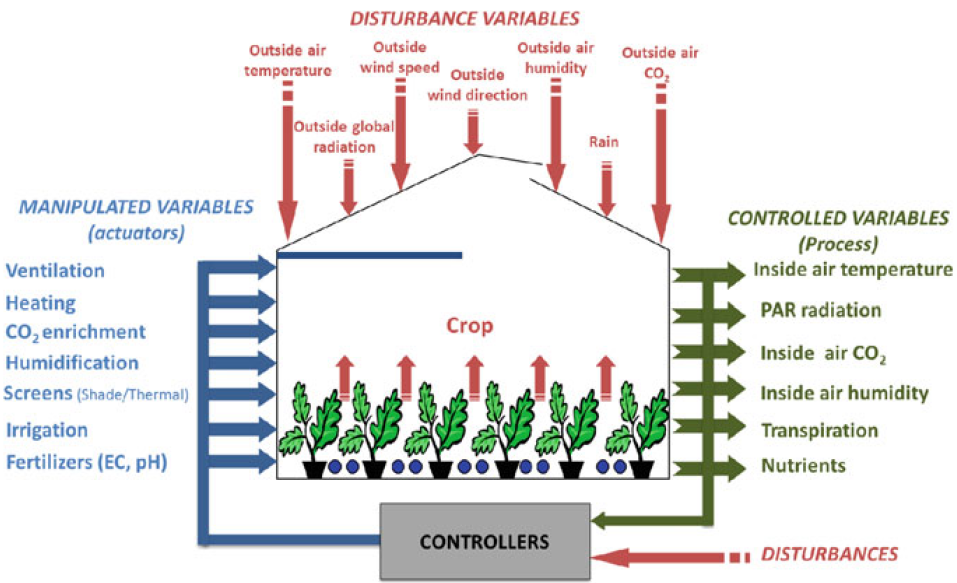
\includegraphics[width=1.0\textwidth]{user-view/climate-control-scheme.png}
    \caption{Greenhouse as a controlled environment with controlled variables and disturbance factors \cite{rod:greenhouse}}
    \label{fig:scheme:greenhouse}
\end{figure}

\subsubsection*{Greenhouse layout and support structures}

The greenhouse's layout is arranged in ways to optimally make use of the available space by densely
arranging the crops.
Since most greenhouses are used for commercial purposes and in this setting the yield per ground
unit is pivotal the goal is to maximize the yield of each plant.\\

In order to archive this goal, the crops are closely planted next to each other in rows
or lanes with just enough room in between to be accessed by workers (figure \ref{fig:lane1}, \ref{fig:lane2}).

\begin{figure}[H]
    \centering
    \begin{minipage}[b]{0.47\textwidth}
        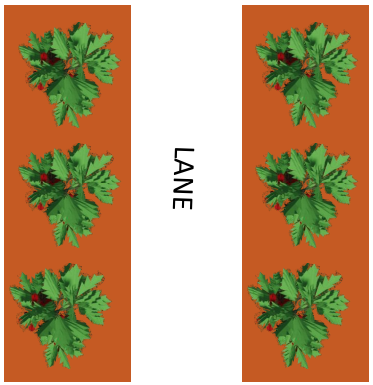
\includegraphics[width=\textwidth]{user-view/lanes.png}
        \caption{Crops arranged in lanes}
        \label{fig:lane1}
    \end{minipage}
    \hfill
    \begin{minipage}[b]{0.49\textwidth}
        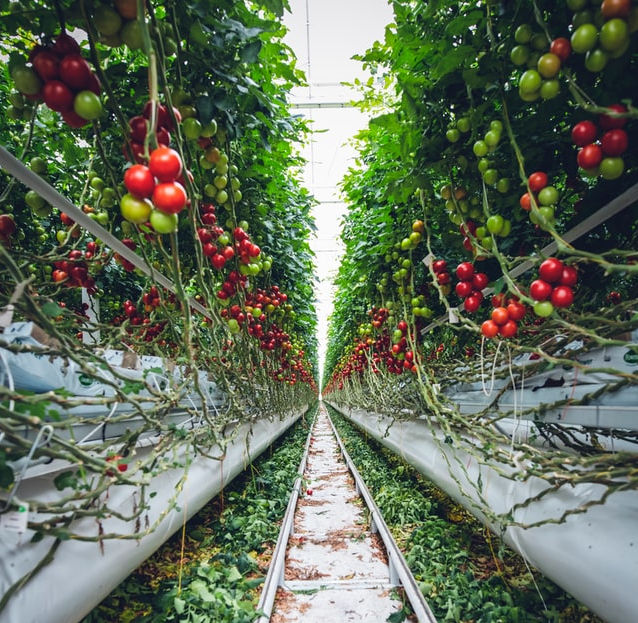
\includegraphics[width=\textwidth]{user-view/plant1_markus_spiske_unsplash.jpg}
        \caption{Walkable lanes}
        \label{fig:lane2}
    \end{minipage}
\end{figure}

Each single plant is supported by a stake which is an effective support structure to ensure
the stability of the tomato plant.
The material and type of the support structure can vary from cage-like structures
to a more common single vertical stake made from any available straight material (figure \ref{fig:stake})
which keeps the plant straight.

\begin{figure}[H]
    \centering
    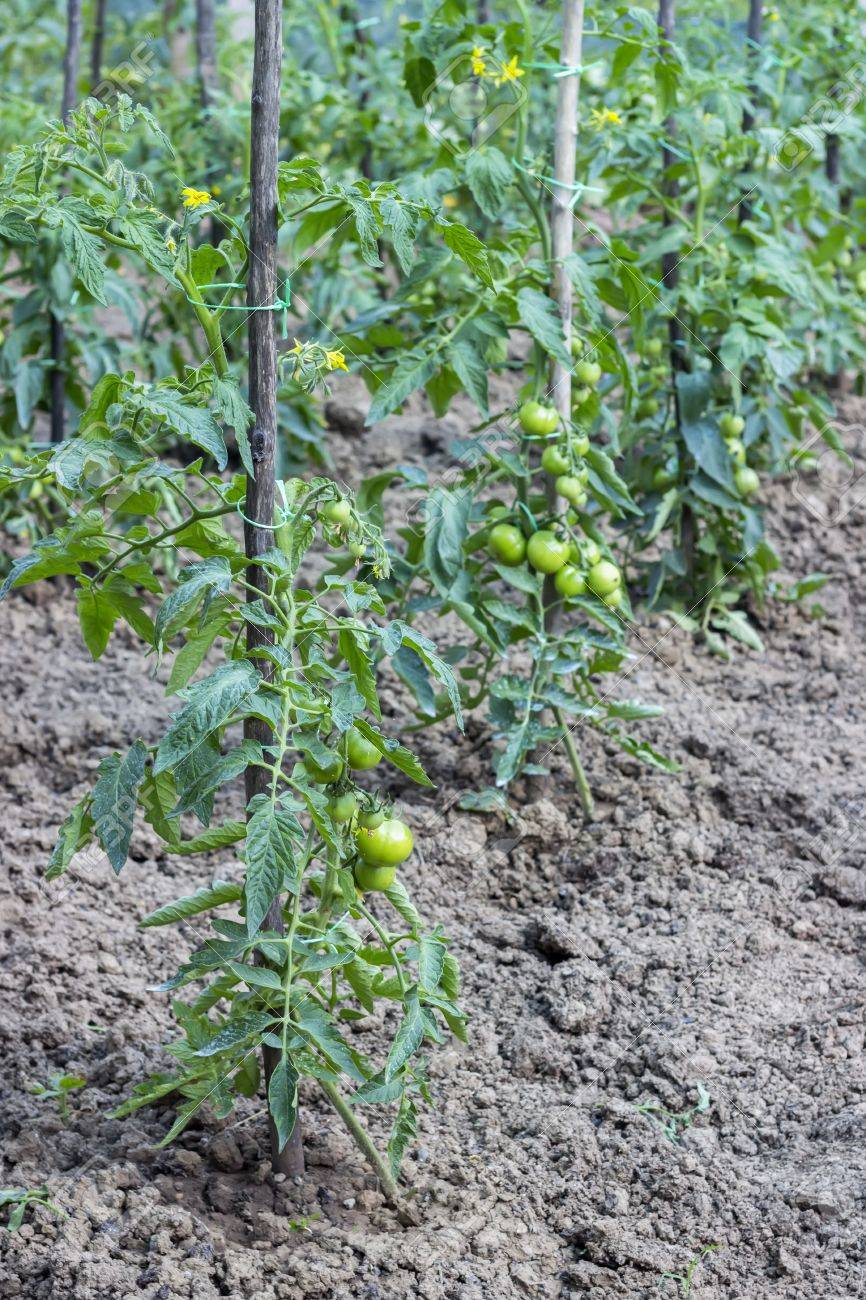
\includegraphics[width=0.3\textwidth]{user-view/tomato_stake.jpg}
    \caption{Plants supported by stakes}
    \label{fig:stake}
\end{figure}

\subsection{Plants}\label{subsec:plants}

This section will give a brief overview of certain aspects of tomato plants physiology
which are important for this project.
Certain physical aspects are introduced and described in more detail in later sections when needed, this
section provides only a brief overview.

\subsubsection*{Growth Stages}\label{sec:growth-stages}

Tomato plants undergo roughly five growth stages throughout their lifetime which are apparent through
physical changes.
Figure \ref{growth-stages} shows the different stages of a tomato plant throughout its lifetime.
The relevant features for our purpose here are the plant's geometric development in each growth stage
and the appearance of certain colors in each phase.

\begin{figure}[H]
    \centering
    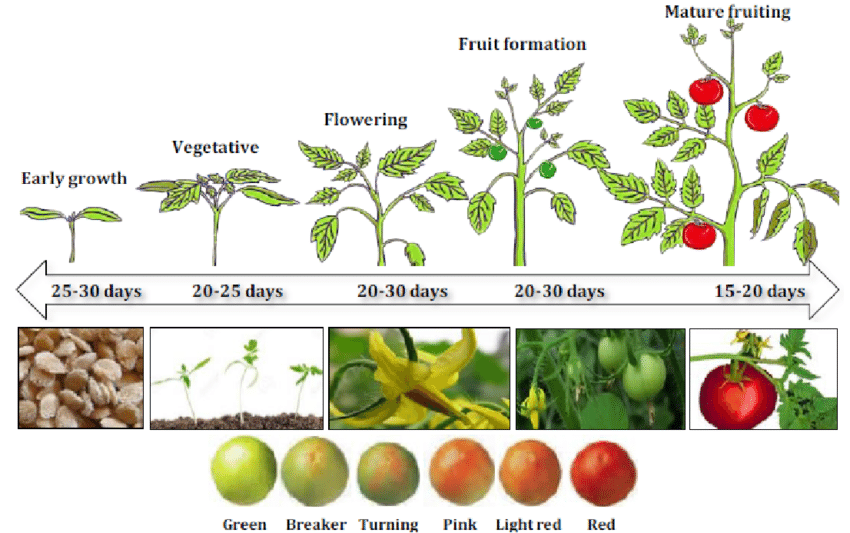
\includegraphics[width=1.0\textwidth]{user-view/growth_stages.png}
    \caption{\enquote{Demonstration of the five growth stages of tomato, and the different levels of fruit ripeness.} \cite{Shamshiri2018}}
    \label{growth-stages}
\end{figure}

In later growth stages, additional branch structures appear above pre-exiting branches creating a level-like
plants appearance whereby older branches are longer and newly grown branches are naturally shorter.\\

Tomato fruits are healthy and ripe once their surface is covered entirely in an rather dark red.
There also exist other varieties of tomatoes which yield to yellow or green ripe fruits but those
or not used here.

\subsubsection*{Leaves}

The main driver for bio-activity in plants is initiated through photosynthetic active radiation (PAR)
through the impact of light on the leaf surface and interaction with gas.
Depending on the growth stage and lighting conditions the leaf surface can appear differently.

In earlier growth stages the leaves are light green and slightly translucent (figure \ref{fig:trans}).
In later growing stages the leaf textures is typically a darker green, hairy and covered
with a wax making the leaves appear mostly mat and dark green (figure \ref{fig:wax}).

\begin{figure}[H]
    \centering
    \begin{minipage}[b]{0.49\textwidth}
        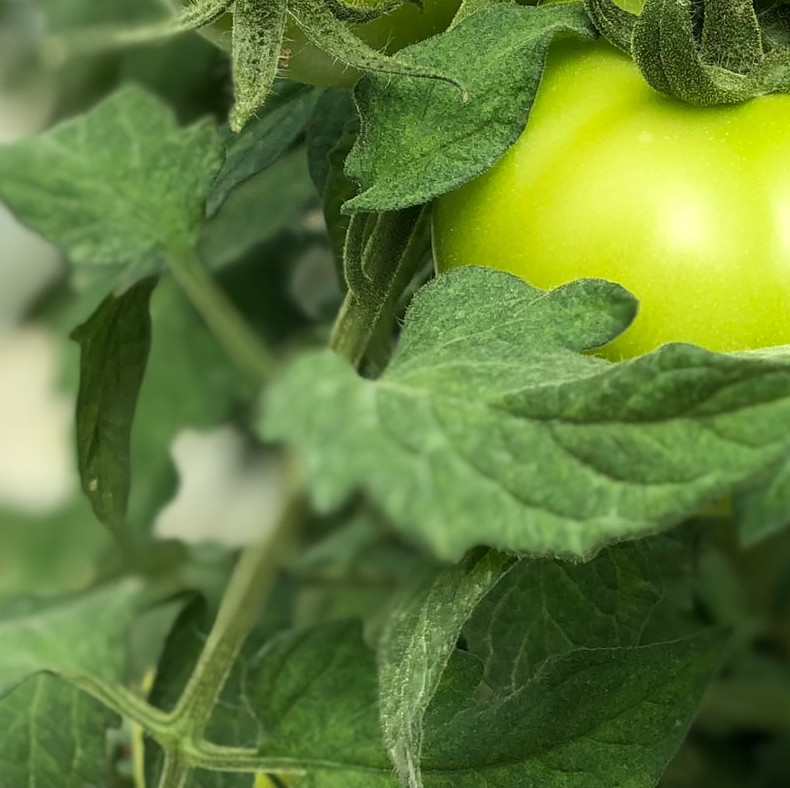
\includegraphics[width=\textwidth]{user-view/plant4_leaf_Soo_Ann_Woon_Unsplash.jpg}
        \caption{Hairy, waxy leaf surface}
        \label{fig:wax}
    \end{minipage}
    \hfill
    \begin{minipage}[b]{0.49\textwidth}
        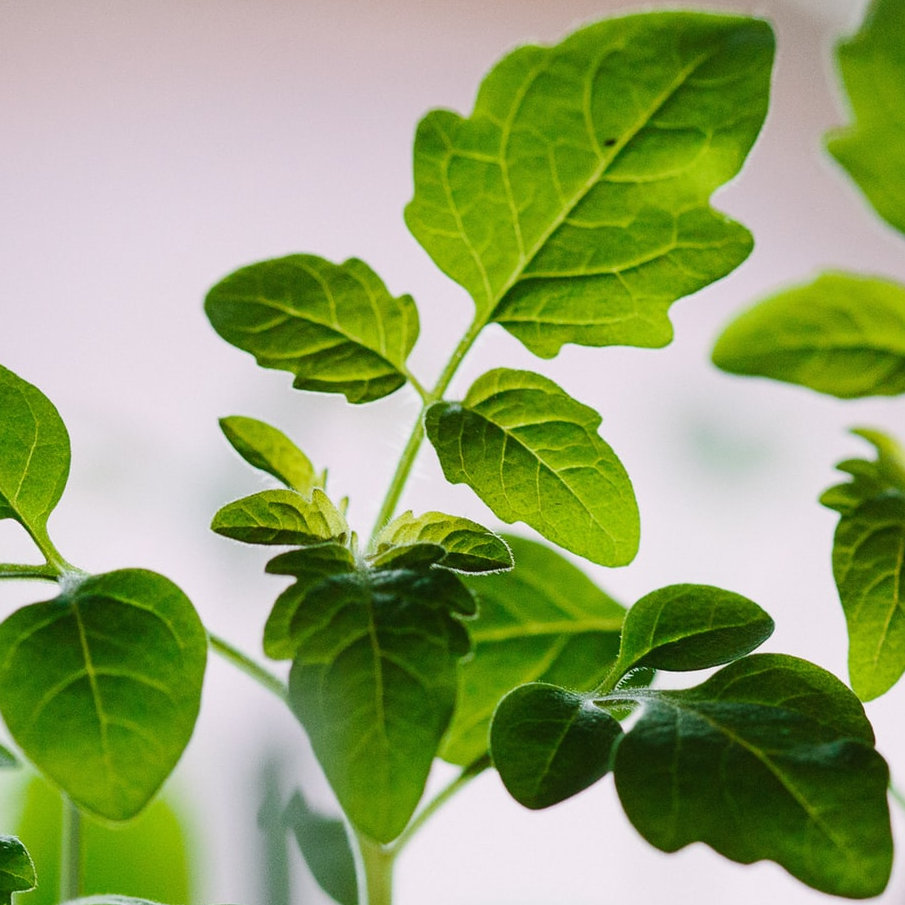
\includegraphics[width=\textwidth]{user-view/plant2_Francesco_Gallarotti_unsplash.jpg}
        \caption{Young leaves partly translucent}
        \label{fig:trans}
    \end{minipage}
\end{figure}

\subsubsection*{Defective Plants}

Defects in plants are either apparent through visibly damaged leaves, fruits or both.
Healthy leaves which contribute to the plant's bio-activity - and hence its yield - are throughout green
and do not contain other colors or physical damages.
Damaged fruits are also apparent through drastic color differences along the surface ,
like red-like and black or red and orange.

Figure \ref{fig:septoria} and \ref{fig:blight} show the two most common diseases which are visible through leave changes and
figure \ref{fig:Anthracnose} and \ref{fig:blossom} and show the two most common fruit diseases - both are caused by fungi
and lead to unusable yield \cite{diseases}.

\begin{figure}[H]
    \centering
    \begin{minipage}[b]{0.45\textwidth}
        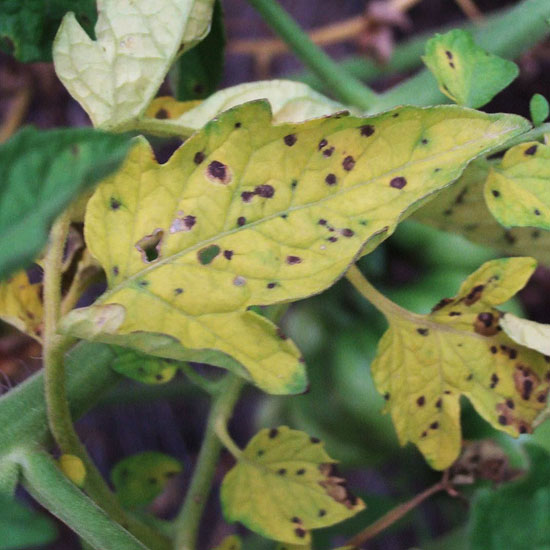
\includegraphics[width=\textwidth]{user-view/sick_0.jpg}
        \caption{Septoria Leaf Spot: Fungus}
        \label{fig:septoria}
    \end{minipage}
    \hfill
    \begin{minipage}[b]{0.45\textwidth}
        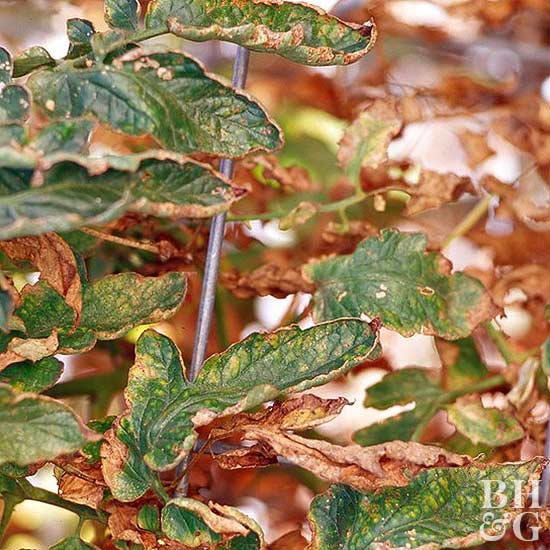
\includegraphics[width=\textwidth]{user-view/sick_1.jpg}
        \caption{Early Blight: Fungus}
        \label{fig:blight}
    \end{minipage}
\end{figure}

As visible the fungi affect leaf surface and color. Both have deviating color and texture
as expected from green healthy leaves.

\begin{figure}[H]
    \centering
    \begin{minipage}[b]{0.45\textwidth}
        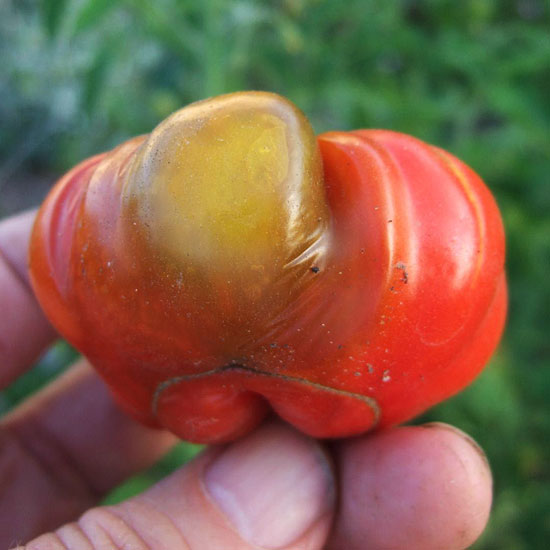
\includegraphics[width=\textwidth]{user-view/sick_2.jpg}
        \caption{Anthracnose: Fungus}
        \label{fig:Anthracnose}
    \end{minipage}
    \hfill
    \begin{minipage}[b]{0.45\textwidth}
        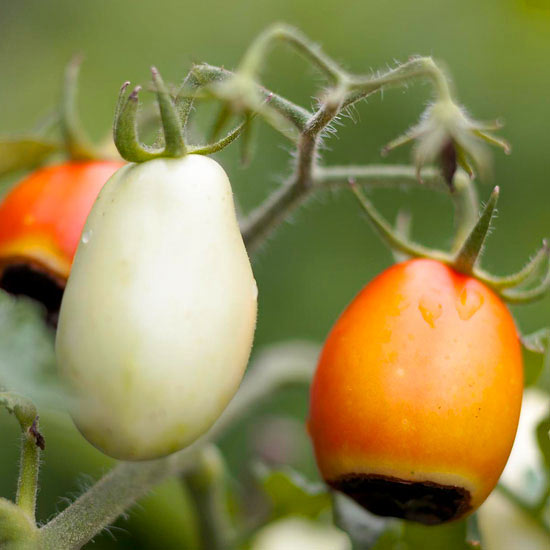
\includegraphics[width=\textwidth]{user-view/sick_3.jpg}
        \caption{Blossom-End Rot}
        \label{fig:blossom}
    \end{minipage}
\end{figure}

Damaged fruits are visible through big differently color clusters along the surface.

\clearpage
\subsection{Task Requirements}\label{subsec:task-requirements}

This project is concerned with the commercial domain of yield production and its purpose
is to predict yield, hence the goal is to design a solution which can automatically estimate yield:\\

For this purpose the requirements are:

\begin{enumerate}
    \item Estimate yield based on camera images taken from tomato plants within a greenhouse
    \item the greenhouse space should be used as effective as possible, means that the number of plants per group unit should be dense
    and ideally no rearrangement is necessary and mainly minimal additional equipment is needed
\end{enumerate}
\newpage


\section{Modeller-View}

The following chapter provides a system design for the task of yield prediction.

The data for the task of yield prediction is solely acquired through photo cameras, hence a system design is
presented which can make prediction by two metrics which are computed from images.
\graphicspath{{members/ssr/figures/modelling}}

\subsection{Design Overview}
\input{members/ssr/authors}

The designed system for the purpose of yield prediction is founded on one central assumption: 
the main metric for vital growth is the leaf area index (LAI) which determines the PAR:

\begin{quote}
    \centering
    Leaf area index (LAI) is the total one‐sided area of leaf tissue per unit ground surface area.
    It is a key parameter in ecophysiology, especially for scaling up the gas exchange from leaf
    to canopy level.
    It characterizes the canopy–atmosphere interface, where most of the energy fluxes exchange. \cite{beda:nathalie}
\end{quote}

For this purpose a plant model is defined in the following section which is used to compute the LAI

\graphicspath{{members/ssr/figures/}}

\subsubsection*{Plant Model}

Based on the physiological description of tomato plants - as provided by the user view - a plant model has
been chosen as shown by figure \ref{fig:plant:model:2}.

\begin{figure}[H]
    \centering
    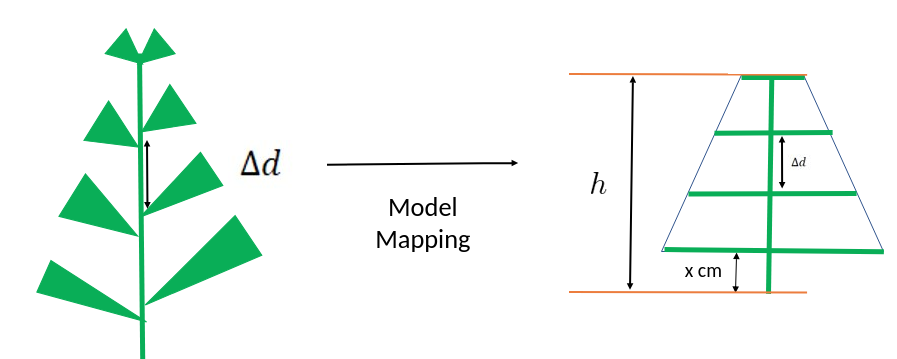
\includegraphics[width=0.9\textwidth,height=\textheight,keepaspectratio]{modelling/plant-model-3.png}
    \caption{Tomato plant model}
    \label{fig:plant:model:2}
\end{figure}

This model especially serves for the purpose of LAI calculation where the canopy visible from above can 
be mapped to the largest (and lowest) branch level of the plant - whereby each higher (and therefore newer)
level is smaller.
The size of the plant's entire leaf area is then correlated with the number of levels.
This model will be formalized in more detail later with all of its parameters. 

\subsection{Computational Pipelines}
\input{members/ssr/authors}

To measure this central metric, two computation pipelines are combined to extract specific metrics from images.
Each pipeline applies a series of image processing and computations in order to contribute to the result
in the following ways:

\begin{enumerate}
    \item \textbf{Pipeline A:} Estimates the \textit{leaf area} (not LAI) which is the visible canopy
    of a single plant, captured by camera mounted above of the plants.
    \item \textbf{Pipeline B:} Estimates the plant height, based on an image taken from a different camera,
    with a specific setup.
\end{enumerate}

Both metrics are then combined (with additional statistical corrections) to estimate the actual LAI.
Again, the LAI is different from the \textit{leaf area} in the way that it contains
the \textit{entire} existing leaf area and not only the leaf area which is visible from above.

\subsection{Pipeline A}\label{subsec:pipeline-a}

Introduce ...

\begin{figure}[H]
    \centering
    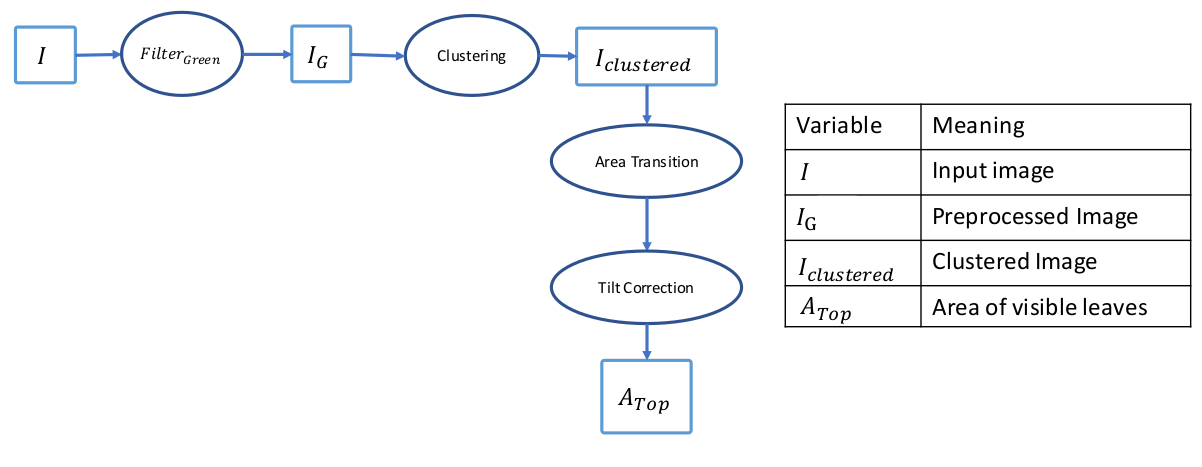
\includegraphics[width=1.0\textwidth]{modelling/pipeline-a.png}
    \caption{The pipeline can be accessed by web browser or purely on a Windows desktop.}
    \label{fig:p:a}
\end{figure}

\graphicspath{{members/ssr/figures/}}

\subsubsection{Camera Setup}
\input{members/ssr/authors}

The input data for Pipeline A is acquired through a digital photo camera which is mounted above the
plants and can move along each lane and take an image from every single plant.
Each captured image contains a square of a ground unit which shows only one plant from above
showing it's canopy, as shown in figure \ref{fig:pipeline:a:camera:setup}

\begin{figure}[H]
    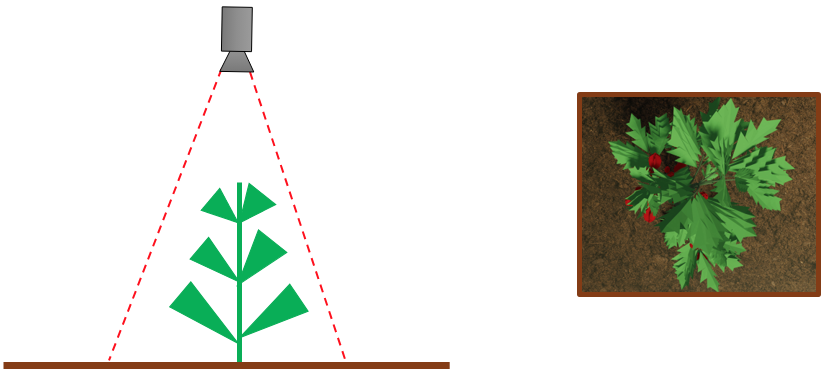
\includegraphics[width=0.9\textwidth,height=\textheight,keepaspectratio]{modelling/camera-setup.png}
    \caption{Camera setup for input data for Pipeline A. Right: Canopy image taken by the camera}
    \label{fig:pipeline:a:camera:setup}
\end{figure}

This basic metric is fed into the pipeline for further processing.
Its purpose is to measure the canopy size which is done by segmentation, as presented in the next chapter.
\subsubsection{Leaf Area Segmentation}\label{subsec:segmentation}
\input{members/ssr/authors}

\textit{Segmentation} here refers to the process of \textit{image segmentation}, which is the process
of partitioning an image into multiple areas or segments which have distinct meanings.\\

In this specific context, the purpose of the segmentation it to distinguish the canopy of one plant
from it's surrounding.

The specific greenhouse layout allows to assume that crops are planted in lanes, next to each other, this
allows to take individual images from above only showing the canopy.

If this constrain is not met, then the presented approach will break, since one plant can't be
differentially from another.

Since individual plants are capture per image the green color dominating areas must belong to the
plant's canopy, hence a simple approach to segmentation can be used by finding all pixel with
dominating green color ratio, which is the case when following condition is true:

\[
    \frac{G + \epsilon}{\max{\{R, B\}} + \epsilon} > 1.0 
\]\\

Where $R, G, B$ are values of each color channels of each pixel, with small $\epsilon$ to prevent division by zero.
High red values indicate either dry leaves or red tomatoes - which are both not part of the leaf
area.
Green tomatoes are also irrelevant since they lie on top of leaves and branches and don't increase
accidentally the leaf area.\\

Once the canopy of a plant can be separated from it's surrounding then the proportion of visible leaf
area from above can be calculated per ground unit which is visible on the image.
The segmented leaf area can then be measured and mapped to the model as illustrated
by figure \ref{fig:mapping}

\begin{figure}[H]
    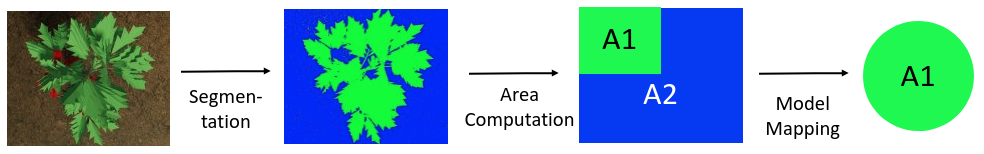
\includegraphics[width=\textwidth,height=\textheight,keepaspectratio]{modelling/mapping.png}
    \caption{Mapping the visible leaf area to lowest level of plant model}
    \label{fig:mapping}
\end{figure}

Once the canopy size is estimated, it can be used in later stages to map it to the plant model.
Figure \ref{fig:canopy} shows the relation between canopy and model mapping.

\begin{figure}[H]
    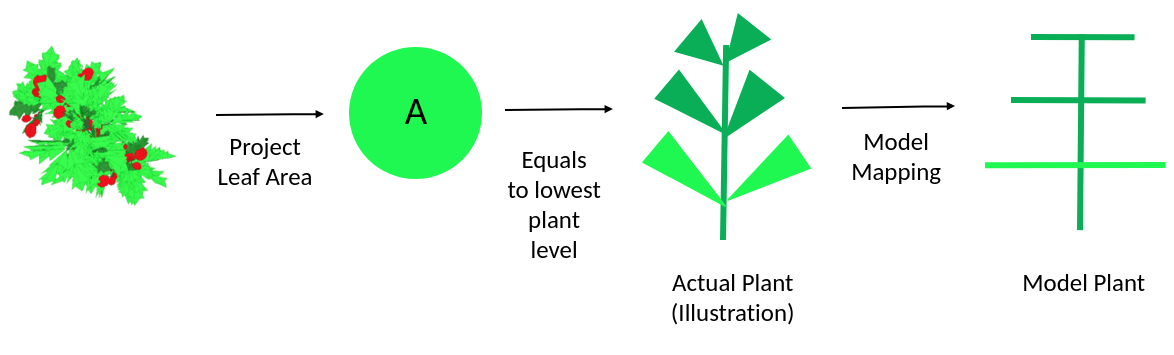
\includegraphics[width=\textwidth,height=\textheight,keepaspectratio]{modelling/plant-model.png}
    \caption{Mapping canopy to plant model}
    \label{fig:canopy}
\end{figure}

As it is obvious, this assumes that the lowest level is the biggest visible area from above
and the number of levels and the size of each level still needs to be estimating for estimating the
entire leaf area.
This will be described in later sections more formally.


\graphicspath{{members/tf/figures/}}

\subsubsection{Area transition}
\input{members/tf/authors}

In previous steps we used clustering to estimate the fraction of pixels in the image from above that display leave surface. But this value is only a fraction and no area measure jet.\\
To translate that fraction into an area we have to find the total area that the camera observes first. To do that we take a look at the camera setup (figure \ref{fig:setupAbove}) again.
   \begin{figure}[H]
       \centering
       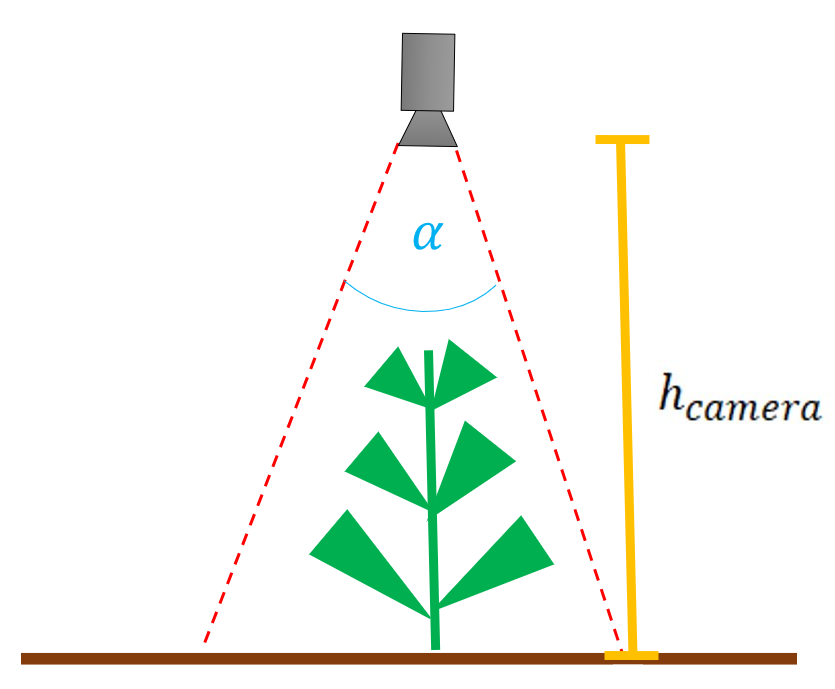
\includegraphics[scale=0.6]{setupAbove.PNG}
       \caption{Setup of the camera above the plant. $\alpha$ denotes the lense angle in which the camera captures the picture. $\alpha$ and $h_{Camera}$ are known.}
       \label{fig:setupAbove}
   \end{figure}
By only looking at half of the cone that the camera covers we can spot a triangle with a $90^{\circ}$ angle. Furthermore the height of the trianlge is $h_{Camera}$, the angle in the upper corner is $\frac{\alpha}{2}$ and the bottom side has a length of half the width of the observed area. The width of the observed area, calculated from the triangle needs to be squared, to get the area of the squared image:\\
$$A_{Camera} = (2\cdot h_{Camera}\cdot tan(\frac{\alpha}{2}))^2$$
$A_{Camera}$ only needs to be calculated once, as long as the camera parameters don't change. To calculate the area of the observed green, we simply multiply the captured area of the camera with the fraction $p_{Green}$ calculated by the clustering: 
$$A_{Observed} = p_{green}\cdot A_{Camera}$$
\textbf{Note:} This whole process works as long as the camera is set as supposed. A tilted camera would break the results since the used triangle would no longer have a $90^{\circ}$ angle. A tilted camera might also unintentionally capture adjacent plants.\\
\textbf{Model:} The observed plants are relatively small (max 40cm) in relation to the height of the camera (min 2m). Hence the plants can be considered to be flat on the ground, without changing the visible area. This assumption breaks when the plants grow much larger than expected. However this is pretty uncommon and can be therfore be neglected.
\subsubsection{Tilt angle correction}
The area calculated in the previous section represents the green area seen from above, which is not the area of the leaves in the canopy we are searching for. That's because the leaves aren't aligned horizontal but tilted and therefore their size is not perfectly captured as seen in figure \ref{fig:tiltedLeaf}. We have to add a correction to the obseved area to estimate the canopy area.\\
   \begin{figure}[H]
       \centering
       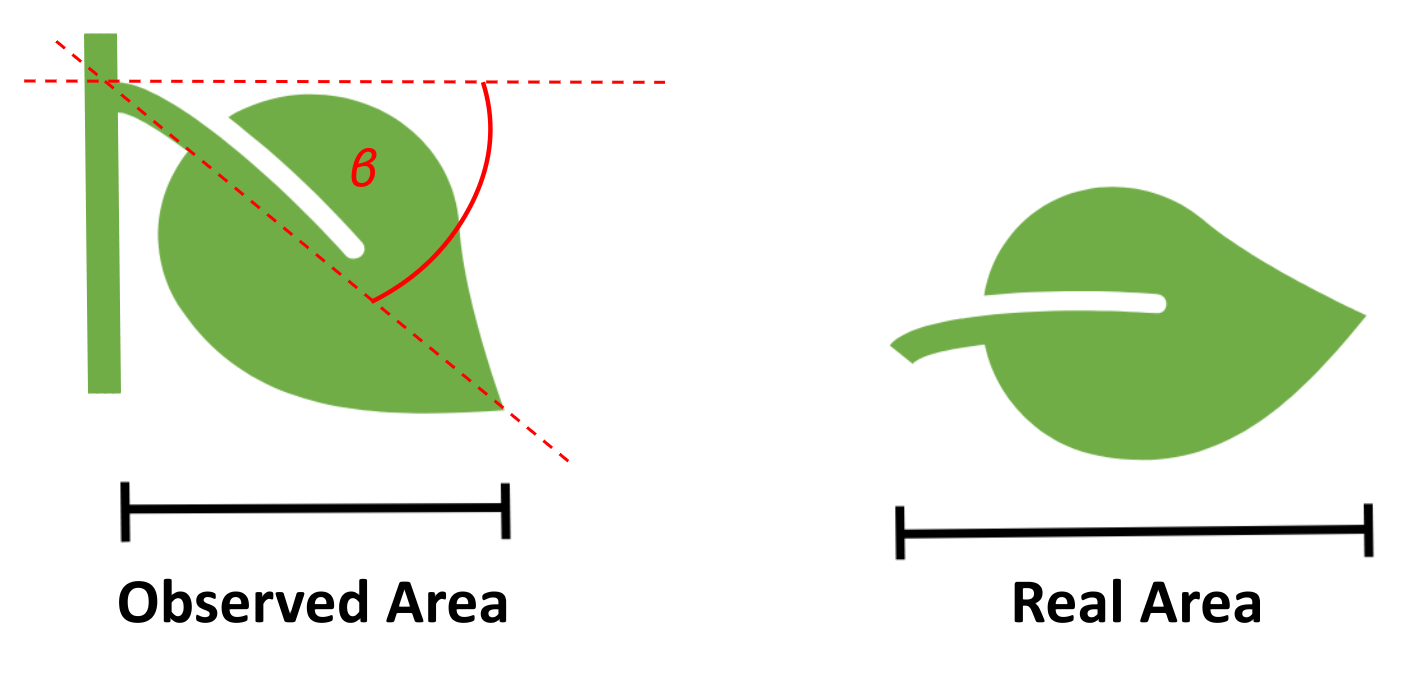
\includegraphics[scale=0.6]{tiltedLeaf.PNG}
       \caption{Sideview comparision of an untilted and a tilted leaf. The captured area from above reduces as a leaf gets tilted by an angle $\beta$.}
       \label{fig:tiltedLeaf}
   \end{figure}
The single leaves are assumed to be uncurved planes, therefore the observed area, the real area and the tilt angle $\beta$ form a $90^{\circ}$ triangle in the 2D sideview. Hence:
$$A_{Canopy} \approx \frac{A_{Observed}}{\arccos \langle |\beta |\rangle }$$
the absolute value of $\beta$ is used in this formula, because wether the tilting is upwards and downwards does not effect the visible area. furthermore the mean of $\beta$ is used, since the single tilt angles of the leaves are unknown and hard to estimate. That mean denotes the mean over all plants, not just a single one. However $\langle |\beta |\rangle$ is still hard to estimate, therefore $\arccos \langle |\beta |\rangle$ is replaced by a parameter that will be trained once the model is in use.\\
\textbf{Model: } The leaves are modeled as uncurved planes, which is most likely not true. Nevertheless the transform described in this section is expected to work, because the trained factor is will not only be trained to correct tiltangles but also curvature of the leaves. Using the model will show whether a linear model can learn this transformation. Assuming that each leaf is scaled by a factor, a linear model should do just fine. Coverage of leaves, which might also occure with adjacent leaves and affect the observed area will also be learned by that linear factor.
\subsection{Pipeline B}
\input{members/tf/authors}
The Area of the canopy, that was calculated in the previous section only tells us about the width of the plant but not the total leaf area. The area alone can not divide the difference between a tall relatively thin plant and a small relatively wide plant as they might have the same canopy green area but a different Leaf Area Index. The same is for a tall plant that is not thin but has large brown areas making the measured canopy small just like a thin plant.\\
Therefore the height gets measured aswell, to capture the size of the plant better. The Pipeline in figure\ref{fig:pipelineB} shows, how a picture from the side is used to determine the top of the plant. First of all an edge detector is applied on the picture. Then the longest edge (the pole behind the plant) is found. To find the top of the plant a small window slides down the post until it detects green covering the pole. That point will be considered as the top of the plant. From that point and the camera setup the height can be calculated. 
   \begin{figure}[H]
       \centering
       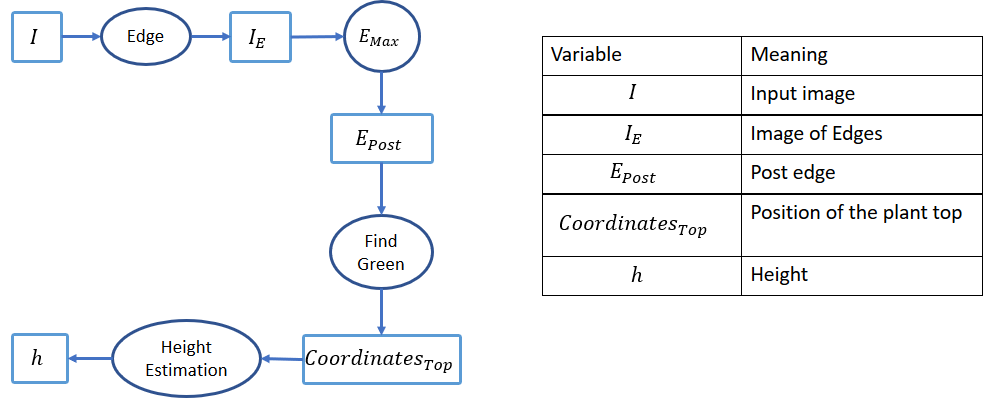
\includegraphics[scale=0.6]{pipelineB.PNG}
       \caption{Pipeline to estimate the height of the plant.}
       \label{fig:pipelineB}
   \end{figure}
\subsubsection{Height estimation setup}
The camera  is set as seen in figure \ref{fig:setupSide}. The camera is set at a certain height ($h_camera$), a certain distance from the plant ($d$) and has a known tilt angle $\alpha$. The camera slides over a rail, that has a constant distance to the plant lanes and a constant height, to make sure the setup stays the same for every plant.
   \begin{figure}[H]
       \centering
       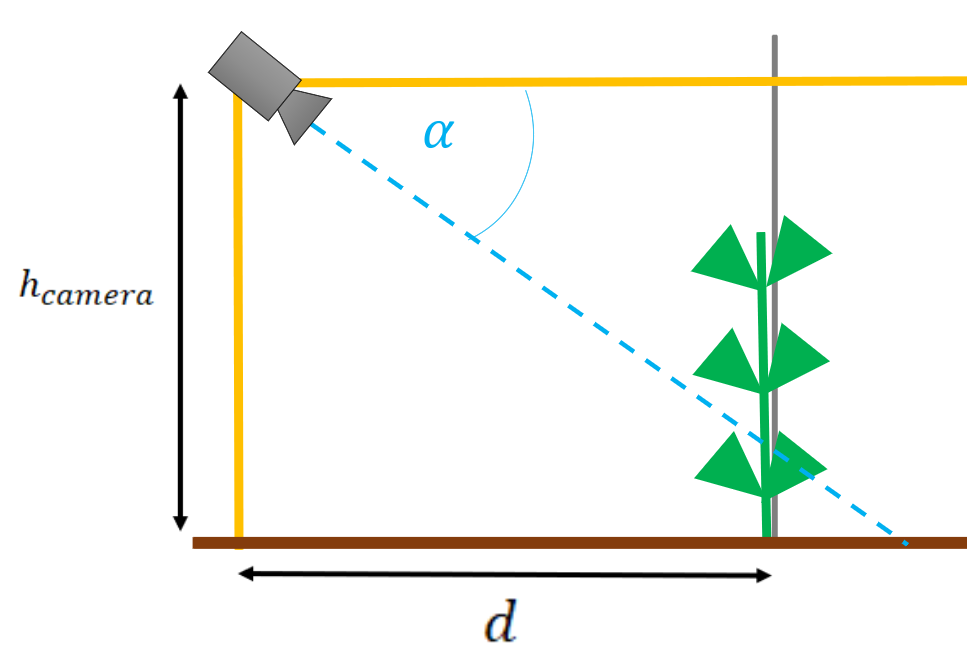
\includegraphics[scale=0.6]{setupSide.PNG}
       \caption{Setup of the camera on the side of the plant. $\alpha$ denotes the tilt angle of the camera as its slightly facing down. }
       \label{fig:setupSide}
   \end{figure}
Furthermore every plant has a pole that is placed behind the plant from the cameras perspective, this helps the plant grow straight one one hand but is also useful for the procedure described below. it is important that the pole is large enough to exit the top of the camera frame and is as straight as possible.
\subsubsection{Estimating top of plant}
To estimate the top of the plant the pole must be found first. that is done using edge detection.
\subsubsection{Edge detection}
to detect the edges a simple vertical edge kernel is applied to the whole picture. This results in a picture $I_E$ with high values for areas with vertical edges and low values for other areas. For the next step all pixels per column are summed up to get a horizontal vector $C$ to get the edge density of each column.
$$C_i = \sum_{j=1}^{y_{range}} I_{E,j,i}$$
The goal of this is to find the column where the pole is, which will create the biggest edges. The problem is this won't result in one big value, but an area with bigger values, because the pole has two sides, creating two edges and the pole might be tilted which will spread the high values over a spacial interval. To still be able to find the post, we transform the horizontal array before searching for the maximum. 
$$C_{i} = \sum_{j=i-k}^{i+k} C_j$$
That way the biggest edge density, caused by the pole can be found by searching the maximum value in $C$. A reasonable k needs to be tested during implementation and maybe trained later.\\
Once biggest vertical edge is found, a little window of $10\times10$ (larger?/smaller?) pixels is laid on the top of the pole, this is done bay putting it on the top of the picture and the position where the biggest $C$ was found. This might not directly hit the pole, since it might be tilted. To be invariant to little tilts in the pole, a correction is applied. If the window covers mostly grey pixels (pole), the pole is found. A threshold for the amount of of grey pixels needed for the window to be considered mostly grey should be tested once the system is implemented. If the window does not cover mostly grey the areas left and right of the window are searched for grey areas that fulfill the threshold. In detail the window is shifted left and right of the original position until a position is found where the threshold is fulfilled. The search for the top of the pole should be limited by a certain distance from the biggest edge to prevent other poles from plants in the background to be found.\\
Once the top of the pole is found, the window starts moving down the pole pixel by pixel. After every step the window is tested to fulfill the threshold, if it does, the search continues with the next step. If the threshold is not fulfilled the window does no longer cover the pole, either because the pole is covered by leaves at that height or because the pole is tilted and the window lost track of it by moving straight down. To prevent the window from losing track of the pole while its still uncovered the same correction is applied that was already used to find the top of the plant, the window searches sideways If it doesn't find a grey area on the left or the right it is because the pole is covered by leaves. Hence the top of the plant is found when the correction can't find a grey area near the old position.\\ 
Once the top of the plant is found by the described procedure the coordinates of the pixel where the search lost track of the pole are stored.
\textbf{Invariances:} The approach with the pole was chosen, to be invariant to green in the background of the picture. That way the plants can be planted close to each other without any problem for this procedure, because no other plant will cover the focused plants pole.\\
The procedure is invariant to slightly tilted poles, since the window is correcting its path every step, but if the pole is tilted to much the top of the pole might not be found. A strongly tilted pole might also affect the results in a negative way since the pole could be entering the plant surface rather from the side than from the top, which would be lower than the top actually is.

\subsubsection{Height estimation}
Once the top of the plant is found in the image, its coordinates need to be translated into the actual height of that plant. To do so we take advantage of our knowledge about the camera setup displayed in figure \ref{fig:estHeight}.
   \begin{figure}[H]
       \centering
       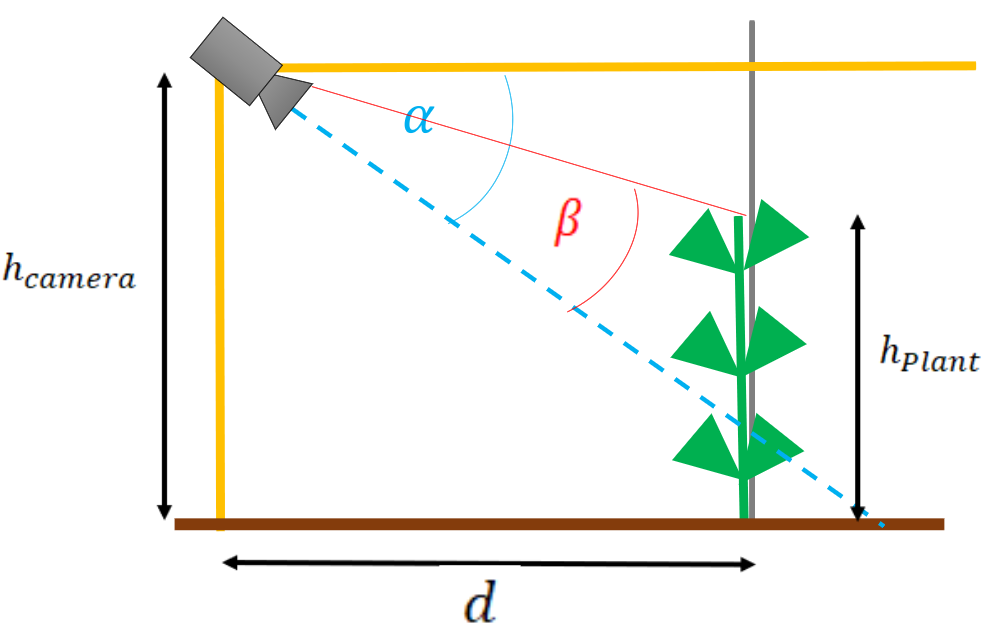
\includegraphics[scale=0.6]{estHeight.PNG}
       \caption{Setup of the camera on the side of the plant. $\alpha$ denotes the tilt angle of the camera as its slightly facing down. $\beta$ denotes the vertical angle between the center of the picture and the top of the plant. }
       \label{fig:estHeight}
   \end{figure}
Once we know the angle $\beta$ we can easily calculate the height of the plant, since we have a $90^{\circ}$ triangle in our setup. The angle $\beta$ is calculated as follows, where $\gamma$ denotes the lens angle, which states the maximum angle the camera captures:\\
   \begin{figure}[H]
       \centering
       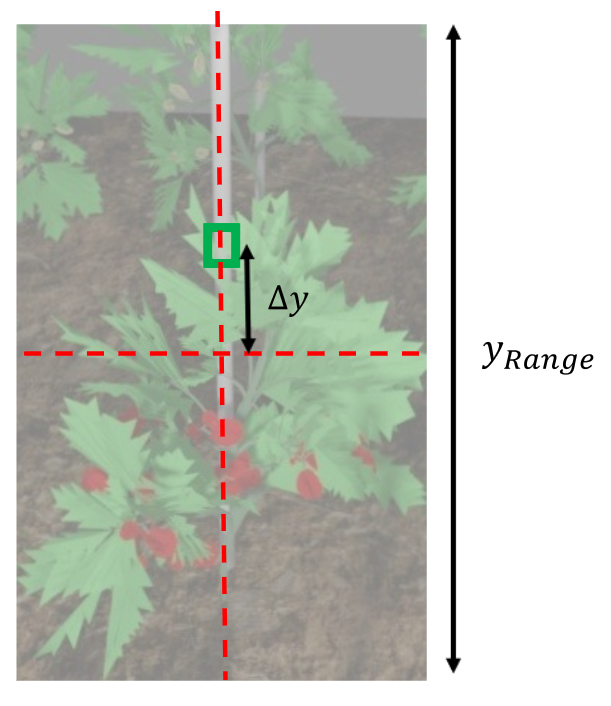
\includegraphics[scale=0.6]{getTopAngle.PNG}
       \caption{$\Delta y$ denotes the vertical distance between the center and the top of the plant in pixels (can be negative if the top is below the center). $y_{range}$ denotes the vertical resolution of the picture.}
       \label{fig:getTopAngle}
   \end{figure}
$$\beta = \frac{\Delta y}{(\frac{y_{range}}{2})}\gamma$$
\textbf{Note:} This works well as long as the picture is not distorted by the lens. Thus its suggested not to use a wide angle lens, since those distort the image unlike regular lenses.\\
Once we know $\beta$ we can calculate the height of the plant :
$$h_{plant} = h_{camera} - d\cdot tan(\alpha - \beta)$$
\textbf{Model:} The model is of the cylinder with levels has a flat area on top (the top level). Hence it is assumed that the first point of the pole that is covered is actually the top. That this idea works quite well is shown in \textcolor{red}{ABSCHNITT IMPLEMENTATION. (STIMMT DAS ?)}
\textbf{Invariances:} a slightly tilted ploe doesn'nt affect this method since the top area of the plant is assumed to be a plane. A strong tilt decreases the precision of the method even if the pole is correctly found, since the pole might enter the plant more from the side at a lower level below the top.
\subsection{Estimating LAI}
\input{members/tf/authors}
\label{section:EstLAI}
After the height of the plant and the canopy area are estimated, they can be used to calculate an estimation for the Leaf Area Index (LAI) which can be used to predict future yield. This combination of the two pipelines is displayed in figure \ref{fig:wholePipeline}.
   \begin{figure}[H]
       \centering
       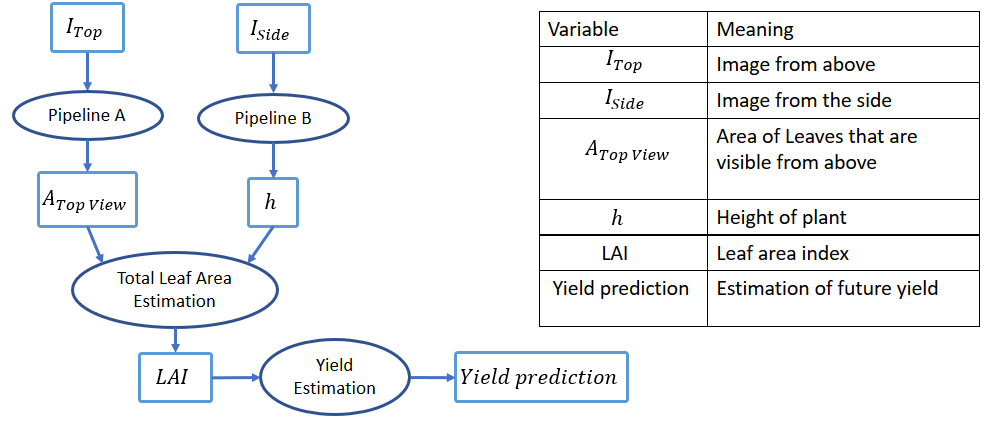
\includegraphics[scale=0.6]{wholePipeline.PNG}
       \caption{Pipeline of the whole process, including the two previously described pipelines.}
       \label{fig:wholePipeline}
   \end{figure}
To calculate the LAI, the green area of the plant is divided by the ground area that it takes part on. Since the ground area is the same for every plant and will be multiplied with a trained factor in section \ref{section:yieldPrediction}, calculating the total green area is quite enough. As already described earlier the plant is modeled as a cylinder with multiple leave levels (see figure \ref{fig:branchRepetition}).
   \begin{figure}[H]
       \centering
       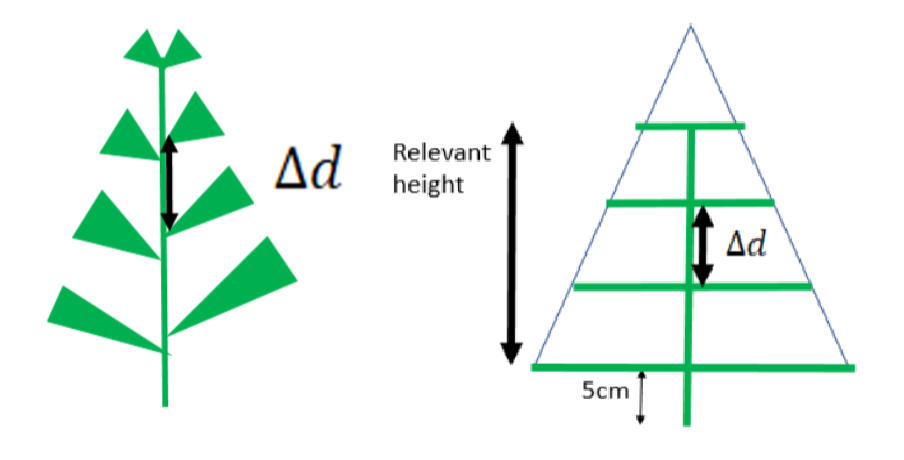
\includegraphics[scale=0.6]{branchRepetition.PNG}
       \caption{Model of the plant (right) consists of multiple levels of leaves with constant distances $\Delta d$ between the levels. The stamp at the bottom of the plant is 5 cm long and has no leaves.}
       \label{fig:branchRepetition}
   \end{figure}
The canopy area measured in pipeline A isdescribes the area of the lowest leaf level of the plant, since that level covers the whole visible area from above. Even though the upper levels partly cover the lowest level, the covered leaves have about the same size as the observed and measured ones.\\
The amount of levels can be calculated by $N_{levels} = \frac{h}{\Delta d}+1$.\\ 
The canopy area is modeled as a circle, like all the levels. Thus a radius can be calculated from the area:
$$r = \sqrt{\frac{A}{\pi}}$$
The radii of the upper levels are linearly decreasing. The area on top of the cone would have an area of zero, which makes sense since the original plant doesn't even reach that high (the cone is one level higher than the original plant).\\ Hence:
$$A_{Total} = \sum_{i=1}^{N_{Levels}}(\frac{i}{N_{Levels}}r)^2\pi$$
The distance of branch repetition $\Delta d$ needs to be trained once the model is in use.
\subsection{Yield prediction}
\input{members/tf/authors}
\label{section:yieldPrediction}
The LAI index has a huge impact on future yield \textcolor{red}{QUELLE?}. The dependecy is assumed to be a non-linear, meaning there is a nonlinear function $F$ s.t. $$yield = F(LAI)$$. To find that non-linearity, data needs to be gathered first. For complex models more data is needed than for simple models. Thus for the first iteration the dependency is assumed to be linear. The yield will then be predicted by
$$yield = m\cdot LAI + b$$
Once much data is gathered and it turned out that a linear model doesn't make good predicitions, it is possible to use more complex models for later iterations.\\
\textbf{Reasonable non-linear approaches:}
\begin{itemize}
   \item Function of higher degree
   \item exponential function
   \item logarithmic function
   \item sigmoid function
   \item neural network
   \item other Machiene Learning methods
\end{itemize}

\graphicspath{{members/paz/figures/}}

\subsection{Summary of Modeler View}\label{subsec:summary-of-modeler-view}
\input{members/paz/authors}

This discussion can be summarized into the following points as input to the
design process:

\begin{enumerate}
    \item The used models focus primarly on estimating yield using only visual information and a stable environmental setting.
    
    \item Each plant being analysed is set constrained to be at a set position with a fixed camera angle to take the pictures. The illumination is constrained by the greenhouse properties and a time given for the data acquisition. So Invariance to camera pose and illumination are not required.
    
    \item The appearence of the object in the image is unconstrained. Invariance to the photometric properties of the plant is a requirement.
    
    \item The Leaf area can be recognized through the green color that is distinguisable from the surrounding ground color. Healthy leaves also appear in a  different green tone then unhealthy or dead leaves. These informations can be used for the design of a model-based approach.
    
    \item Information on exact values (green color treshhold, leaf level distance) can be refined via data-driven learning approaches.
    
\end{enumerate}

\subsection{Requirements to Modules Choices}
\input{members/paz/authors.tex}

\subsubsection*{Component selection}

The requirements to module choices motivate the use of model-based and data-driven components. In this implementation of the project the focus lies on model based component choices. In the following we enumerate the link between module choices and model.

\begin{enumerate}
    \item \textbf{Constrained information Input:} Due to the fact that the amount of information gathered is limited to visual information, the choosen modules need to estimate the wanted information as accurate as possible. We choose the LAI (Leaf area index) as the parameter due to the strong correlation to yield \cite{heuvelink2004effect} and the possibility to gather this parameter using image processing.

    \item \textbf{Mensuration exploits contextual priors:} The mensuration module can exploit the greenhouse setting in the acquisition setup, i.e. the cameras are set at a fixed angle and distance from the plant. We know information about the height of the camera and the center point. The intrinsic camera calibration is assumed to be known.

    \item \textbf{Optimizing defect detection:} The Image segmentation model is set up to be variable and adjustable to different toness of green. This enables the module to adjust to changes in the leaf color and detect sick or dead leaf structure. The segmentation at the same time is deviced to be able to match different lighting situations and plant defects by adjusting the green threshold.

    \item \textbf{Scalability, Extensibility of modules to Novel Settings:} The strong modulation of the application allows the option to split, rearrange and reuse specific modules in novel settings.
\end{enumerate}

\subsection{Discussion on Strengths/Limitations of the Leaf Area Index model}
\input{members/paz/authors.tex}

As mentioned above the LAI index gives us a good representation of the PAR (photosynthetically active radiation) which highly influences biomass as well as yield production. \cite{hossain2017leaf} The yield predicted using the above mentioned modules is a useful when the plant is in a full grown state before starting to produce yield, we are able to estimate future yield using the LAI at the moment of time the image is taken. Yield predicitons made by this application are used to estimate yield in the near future. In addition the approximation for full grown tomato plants is robust to inaccuracies. This is explained by the saturation of radiation that can be absorbed.The intercepted light shows a saturation at a specific LAI value. Due to the nature of the project being autonomous to a certain degree the plants do not get unnecessary leaves removed and these leaves are included in the estimated LAI. So the correlation between the LAI and the intercepted light is represented in a flattening curve. See in \ref{fig:LaiCurve}\\

\begin{figure}[h]
    \centering
    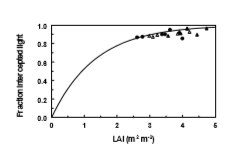
\includegraphics[scale=1.2]{LAI.PNG}
    \caption{\textit{Note: Measurements from \cite{heuvelink2004effect} showing the Fraction intercepted light as function of measured leaf area index (LAI), determined once per month starting from mid-March until mid-August for three leaf picking strategies: reference, high and maximum LAI.  Curve equation: fract. intercept. = 1-e-0.75 LAI.  Each data point based on 3 plots}}
    \label{fig:LaiCurve}
\end{figure}\\

Under following conditions the method would fail:

\begin{enumerate}
    \item When the plant doesn't grow in the intended position it is not possible to estimate the accurate height of the plant and the canopy size and plant height will be esimated with false values. The module will follow wrong assumptions to predict the leaf area and will not be able to give an accurate estimation of future yield.

    \item If the plant shows some abnormalities to the assumed norm. If the leaf density is abnormal low or high in any level of the plant the approximated yield will deviate from the intended value.

    \item Different morphology can not be recognized by the system and will be treated as the assumed cone shaped plant structure.
\end{enumerate}

\newpage
\graphicspath{{members/ssr/figures/}}

\subsection{Integration with Simulation}\label{subsec:integration-with-simulation}

The way in which the entire project was conducted led to some limitations in the way the simulation was executed
which has to be explained in order to understand how it affected the modelling and simulation.\\

Normally, the modelling should be completed (or nearly finished) so that the requirements for the simulation are known.
The reason is that the model must first be formally defined with all of its parameters and then the evaluation can start
on how to simulate the model's parameters accurately - either by using existing tools or by creating them. 
This on its own turned out to be an elaborate enterprise which could not be conducted thoroughly, so a
compromise has been found.

In order to fulfill the time constraints of this project the modelling and simulation team worked in parallel
to evaluate usable simulation tools and this affected the choices made by the modelling group in order
to archive a compromise between a \textit{preferred} and \textit{practical} solution.

The reasons are that the relevant metrics and data gathering setup were not known until later in the modelling
since many approaches had to explored until one promising design was found.

Since the model only relies on leaf area and height measurements, the parameters of chief interest for simulation
were proper simulation of the plant's leaves and the height.

Other factors, like accurate fruit simulation and further probability distributions could not be simulated
since no data has been found or no formal method for gathering conducted, like for leaf tilt distributions.
How to gather such distributions is also another enterprise on its own and won't be investigated here
further.

It was also unclear until later in the modelling that the fruit properties (like texture and color)
were not of chief interest - for the purpose of yield estimation.
Hence, the fruits have only been rudimentarily simulated for testing purposes
- however the fruit properties have not yet been integrated into the model but only used in
data preparation, like segmentation and for this purpose they served well.\\

Following metrics has been selected for the simulation and can be provided with data (or need yet real-world probability distributions):\\

\begin{table}
    \centering
    \begin{tabular}{ |l|l| }
        \hline
        $\theta_{col,leaf}$ & Leaf area color distribution (rough approximation, not exact yet) \\
        $\theta_{col,earth}$ & Non-leaf area color distribution (rough approximation, not exact yet)  \\
        $\theta_{tilt}$ & Leaf tilting \\
        $h$ & Plant model height  \\
        $\Delta d$ & Plant model level distance \\
        %$h_{leaf}(level)$ & Leaf count distribution per level (or per-level leaf density) \\
        \hline
    \end{tabular}
    \caption{Simulation parameters}
\end{table}
\newpage

\section{Simulation}

In order to use the previously proposed models, pictures of tomato plants are required. Since we do not have a greenhouse in which we can take the pictures, a simulation will be used instead. Tomato plants grow according to a pattern. The leaves have a certain shape and the flowers have a certain amount of petals in a certain color. But still each plant is individual, as parameters like the number and position of branches can vary. The simulation should be able to automatically generate a multitude of tomato plants varying in these parameter. Each parameter has a certain range in which it can be selected.

Since we decided to focus the project on the prediction of the amount of leaves on the plant, the simulation of diseases and ripeness becomes secondary. While, we will still explain how these parts could be simulated in general, we will concentrate on the simulation of different amounts of leaves on the plants.  
\graphicspath{{members/cm/figures/}}

\subsection{Building the foundation of the tomato plants}
\input{members/cm/authors}

The goal of the simulation is to create a variety of different realistic tomato plants. The first step is therefore to determine which parameters describe a realistic tomato plant. A tomato plant can be split in four major parts; stem, leaves, flowers, fruits. Each of which, have their own properties, which can vary from plant to plant in a certain range. For example, if a tomato plant carries ripe fruits these are red, round and have a certain size. But how ripe the fruits are and the health status of the plant, can lead to variations in size and color of the fruits. And the amount and position of the fruits are variable, as well. 

In order to create this variability PlantStudio is used.
PlantStudio is a parameter-driven simulation tool, which can be used for the simulation of various non-woody plants throughout their life cycle.
It provides various parameters concerning the structure and the growth of the plant.
It starts with a collection of questions regarding the optics of the plant, containing information about the stem, leaves, flowers and fruits.
This enables an individual adjustment of color, shape, amount and distribution for each of these plant parts. A detailed descriptions of the settings used in this project can be found in table \ref{tab:parameters_plantStudio}. Thanks to the randomize function provided by PlantStudio a multitude of different plants with these parameters can be created.\\

For each created plant PlantStudio animates a life cycle going from the spearing of the plant to the full-grown tomato plant with ripe fruits. The duration of the life cycle and at which point the fruits start to grow, can be manually adjusted to create a realistic representation. \\

\begin{longtable}[c]{@{}p{0.15\textwidth}p{0.45\textwidth}p{0.4\textwidth}@{}}
	\caption{General parameters set in PlantStudio describing the growth behavior of tomato plants.}
	\label{tab:parameters_plantStudio}\\
	\toprule
	& Description                                                                                                                                                                                                                 & Settings                                                                                                                                                                      \\* \midrule
	\endhead
	%
	\bottomrule
	\endfoot
	%
	\endlastfoot
	%
	Meristems               & Meristems are buds from which leaves and branches grow.                                                                                                                                                                     & \vspace{-25pt}
	 \begin{itemize}
		\item opposing to each other \vspace{-10pt}
		\item medium amount of branches \vspace{-10pt}
		\item secondary branches \vspace{-10pt}
		\item angle stem/branch: medium \vspace{-10pt}   
	\end{itemize} \\
	Internodes              & Internodes are portions of plant stem between leaves and determine how short or tall, straight or viney, and stiff or flexible the plant will be                                                                            & \vspace{-25pt}
	\begin{itemize}
		\item long \vspace{-10pt}
		\item medium thickness \vspace{-10pt}
		\item introduce some curve to the plant \vspace{-10pt}
	\end{itemize} \\
	Leaves                  & Leaves are drawn using a 3D-object. The leaf is drawn bigger as the plant grows. Leaves are connected to the plant by a stalk called petiole& \vspace{-25pt}
	\begin{itemize}
		\item pre-build shape: tomato leaf\vspace{-10pt}
		\item small size \vspace{-10pt}
		\item petiole of medium length \vspace{-10pt}
		\item angle stem/leaf: large \vspace{-10pt}
	\end{itemize} \\
	Compound leaves         & A compound leaf contains $>$=2 leaflets. Leaflets look like small whole leaves, but fit together in the same pattern for all leaves of the plant. A leaf without leaflets is a simple leaf & \vspace{-25pt}
	\begin{itemize}
		\item pinnate leaves (seven leaves are ordered feather like) \vspace{-10pt}
		\item leaflet are in a medium distance to each other \vspace{-10pt}
	\end{itemize} \\
	Inflorescence placement & An inflorescence holds fruits and flowers on a plant. It is divided in apical, which means at the end of the plant stems and axillar, which means between the angles between the stem and the leaf.         & \vspace{-25pt}
	\begin{itemize}
		\item no apical inflorescence \vspace{-10pt}
		\item multiple axillary inforescneces (10)\vspace{-10pt}
		\item primary stems have a medium length\vspace{-10pt}
	\end{itemize} \\
	Inflorescence drawing   & Inflorescence can have a variety of shapes                                                                                                                                                                                  & \vspace{-25pt}
	\begin{itemize}
		\item 10 flowers per inflorescence\vspace{-10pt}
		\item placed in spikes\vspace{-10pt}
		\item stem thickness:  medium\vspace{-10pt}
	\end{itemize} \\
	Flowers                 & Like leaves flowers are drawn as 3D objects, with each 3D object representing one petal of the flower.                                                                                                                      & \vspace{-25pt}
	\begin{itemize}
		\item 4 small, yellow pedals\vspace{-10pt}
		\item pre-built shape: corn leaves\vspace{-10pt}
		\item elongated and pointy\vspace{-10pt}
	\end{itemize} \\
	Fruits   & Fruits are drawn like flowers, but with a portion of fruit rotated around instead of petals                                                                                                                                 & \vspace{-25pt}
	\begin{itemize}
		\item common fruit section 1\vspace{-10pt}
		\item 10 fruit sections per fruit\vspace{-10pt}
		\item huge size\vspace{-10pt}
		\item unripe fruits: green\vspace{-10pt}
		\item ripe fruits: red\vspace{-10pt}
	\end{itemize}
\\* \bottomrule
\end{longtable}


\begin{figure}[ht]
	\centering
	\begin{subfigure}{.24\textwidth}
		\centering
		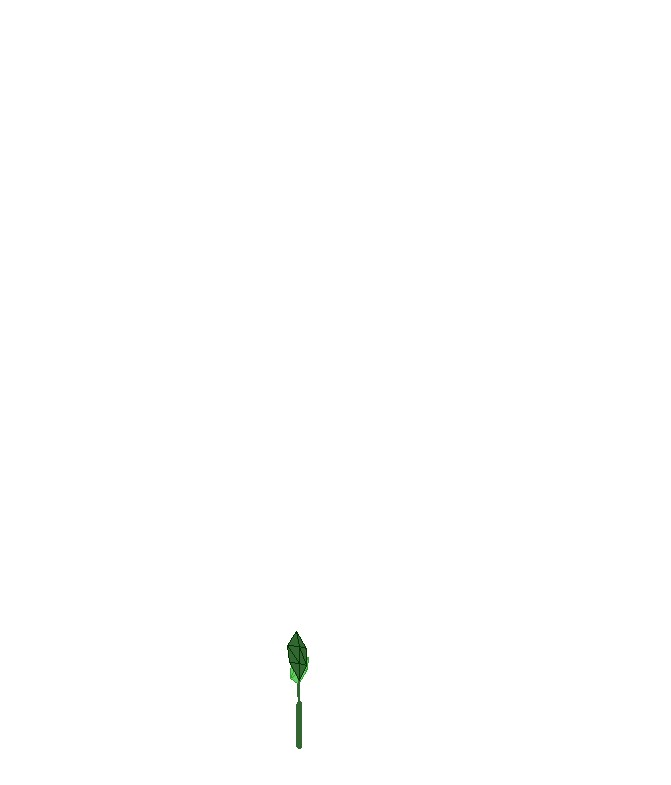
\includegraphics[width=\linewidth]{plantAging001.jpg}
		\label{fig:sub1}
	\end{subfigure}
	\begin{subfigure}{.24\textwidth}
		\centering
		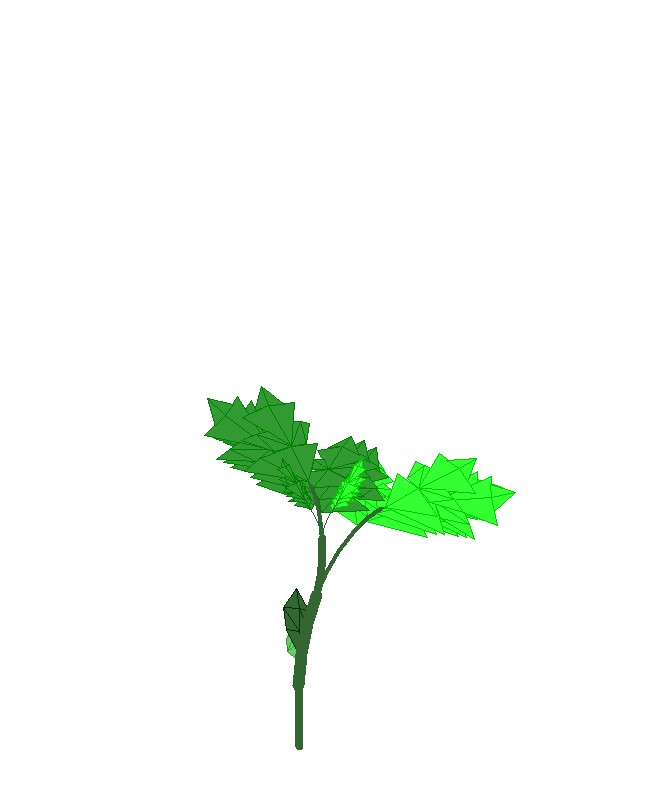
\includegraphics[width=\linewidth]{plantAging002.jpg}
		\label{fig:sub2}
	\end{subfigure}%
	\begin{subfigure}{.24\textwidth}
		\centering
		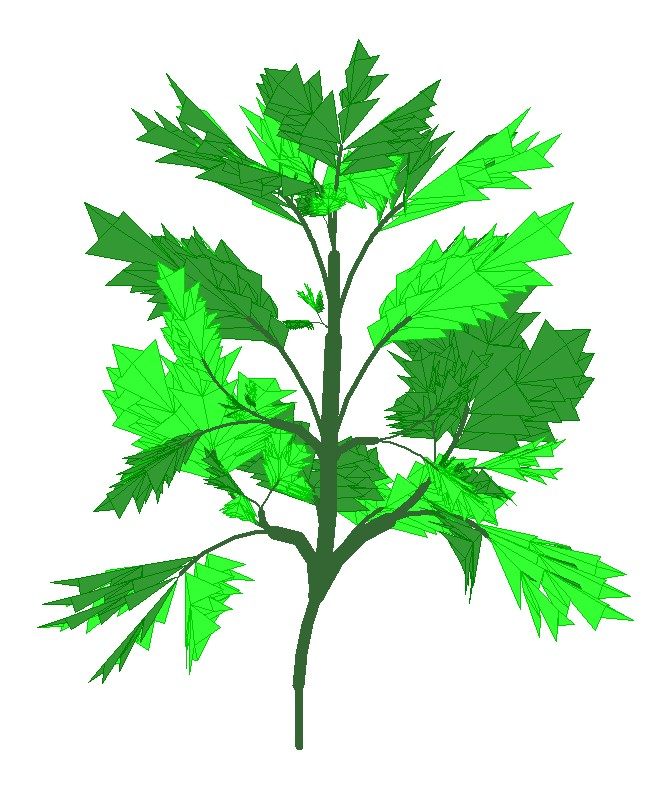
\includegraphics[width=\linewidth]{plantAging003.jpg}
		\label{fig:sub3}
	\end{subfigure}%
	\begin{subfigure}{.24\textwidth}
		\centering
		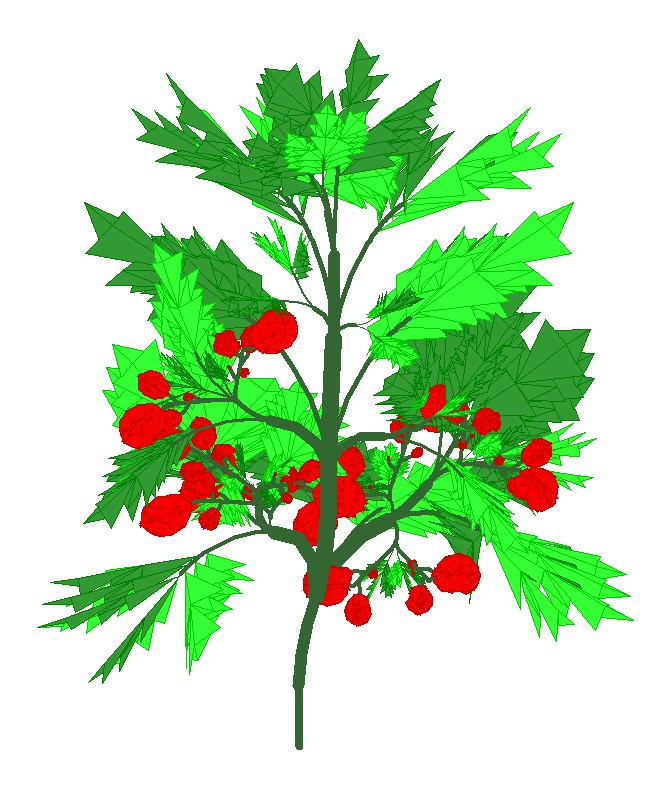
\includegraphics[width=\linewidth]{plantAging004.jpg}
		\label{fig:sub4}
	\end{subfigure}%
	\caption{Example of a tomato plant created with PlantStudios in four different stages of growth}
	\label{fig:plantStudio}
	\vspace{-10pt}
\end{figure} 


The created plants have the general parameters of tomato plant but do not look realistic thus far, which can be seen in figure \ref{fig:plantStudio}. The shortcomings of the simulation, like the missing texture and material, can be solved by using a second simulation tool, like Blender. This is enabled by PlantStuios option to export the plants as wavefronts (.obj). Here, we created a total of 42 different plants, which were saved grouped by individual plant parts, which allows to change each leaf, fruit or flower individually in later steps.



\subsection{Importing and placing plants in Blender}
\input{members/cm/authors}
\begin{wrapfigure}{r}{0.5\textwidth} 
	\vspace{-25pt}
	\begin{center}
		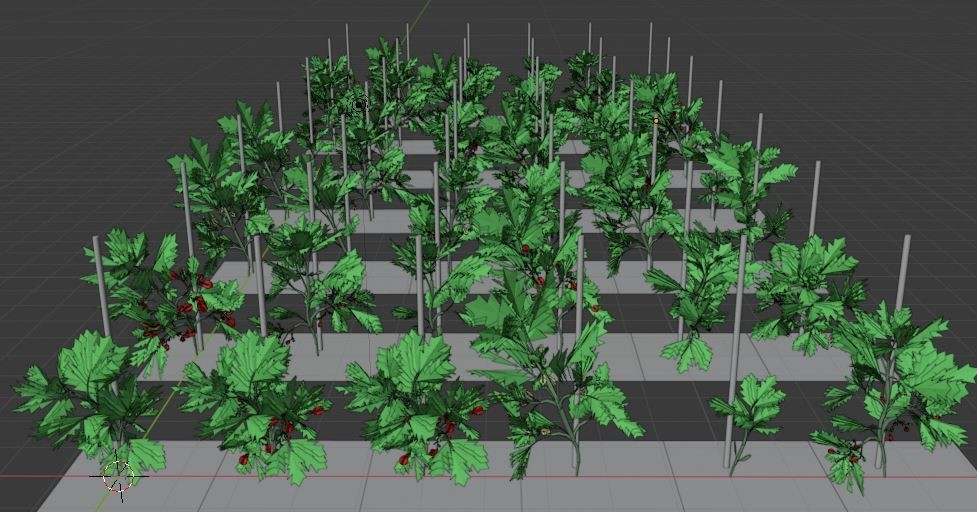
\includegraphics[width=0.45\textwidth]{BlenderImport.JPG}
		\caption{Import of 42 randomly selected plants into Blender with 6 plants per row and soil and pole for each plant.}
		\label{fig:BlenderImport}
	\end{center}
	\vspace{-20pt}
	\vspace{1pt}
\end{wrapfigure} 

The tomato plant can be imported into Blender. Blender is an open source computer graphics software, which can be used for visual effects, 3D models, etc. The purpose of using Blender is to import the in PlantStudio created plants and  add details, shading, rendering and lighting. The script written to import the plants can be easily adjusted in the number of plants that should be planted and the number of plants that are planted in each row. Which plants are planted is randomly selected from the 42 plants exported from PlantStudio.

\lstinputlisting[language=Python, linerange={12-14}, frame=single, caption = Given a folder \textit{directory\_im} containing obj files a specific number of plants are randomly selected ]{members/cm/import_plants.py}\vspace{5pt}


The plants are than imported and placed in multiple rows of a specific length, that can be set by the user. Here, it is important to select to split the geometry by group, in order to individually adjust each leaf or fruit section. In order to be able to differentiate between the various plants, each plant is placed in its own collection. 

\lstinputlisting[language=Python, linerange={21-39}, frame=single, caption = Inorder to place the plants like they would be placed in the greenhouse we need to know how many plants should be planted and how many fit in one row.]{members/cm/import_plants.py}\vspace{5pt}

Each plant is positioned next to a pole to fix it and on a square of soil. In this step we add these features without any texture and material. These will be added at a later point to further increase the closeness to reality. 

\lstinputlisting[language=Python, linerange={43-49}, frame=single, caption = Placement of the pole next to each plant. Placement of soil is don analog]{members/cm/import_plants.py}\vspace{5pt}


\graphicspath{{members/nh/figures/}}

\subsection{Simulation Part Niusha}
\input{members/nh/authors}

A texture appears on the surface of the meshes and representing the look and material of an object. Ameshis a collection of vertices, edges, and faces that describe the shape of a 3D object.Here we used a texture of a soil which is downloaded from www.texture.com. The advantage of using texture vs. image is that it is not necessary to place the image on each coordination to make it look 3D. Scripting is usedto automate the process of creating and placing nets under each plant. plane = bpy.context.selected_objects[0] print('\nPlane coordinates: X: ' + str(plane.location.x) + ' Y:'+ str(plane.location.y) + '\n') mat=bpy.data.materials.new('materialA') bpy.context.object.data.materials.append(mat) mat.use_nodes = TrueLinked nodes using BSDF principal are defined, which is used for shading textures. bsdf = mat.node_tree.nodes["Principled BSDF"]The downloaded Texture is going to import on each material. texImage = mat.node_tree.nodes.new('ShaderNodeTexImage') texImage.image = bpy.data.images.load("C:/My Documents/Blender/Textur.jpg") mat.node_tree.links.new(bsdf.inputs['Base Color'], texImage.outputs['Color'])ImageImageImageLichtThere is a light source above each plant. Light in Blender 2.8 changed from the name lamp to light.There are ... types of light :Point light is a directional point of light. The light power and size can be easily changed. The power is in Watt and the point light with a larger size has softer shadows and specular highlights.# create light datablock, set attributes light_data = bpy.data.lights.new(name="light_2.80", type='SPOT') light_data.energy = 50 # create new object with our light datablock
 light_object = bpy.data.objects.new(name="light_2.80", object_data=light_data # link light object bpy.context.collection.objects.link(light_object) # make it active  bpy.context.view_layer.objects.active = light_objectImageSpot light is a cone shape beam of light. Just like point light the power of the light is in Watt and the larger size has softer shadows and specular highlights.Area light simulates light originating from a surface. This kind of light is like TV screen or window. Beside the power it also has properties shape and size. The shape of Area light can be rectangle, square, disk, ellipse and the size is defined the dimensions for the square and rectangle.
Sun light provides light of constant intensity emitted in a single direction from infinity far away. It is represented by a encircled black dot with dots emitting from it.


\graphicspath{{Pictures/}}

\subsection{Properties of Leaves}
\input{members/kh/authors}
To achieve more realistic leaves, the simulation receives information from the modeler which analyses the structure of the different parts of the tomato plant. Since the estimation and measurements mainly focus on the leaves, the first structure analysis also just takes the leaves into account.
In the following paragraphs the leaf structure will be analyzed. First it is only looked at three structural aspects. If this approach is not meaningful after designing there are more parts that need to be analyzed later on.

\subsubsection{Color}
The green color of a leaf comes from clorophyll. It a class of natural coloring which is produced by different organisms. 
The absorption spectrum of clorophyll is shown in Figure \ref{clorophyll}. It is shown that all wavelength accept 500nm to 600nm is being absorbed. The green color is a sign for a well functioning  photosythesis. This leads to the conclusion of a good growth and a healthy plant. Therefore healthy plants appear in a green color.

\begin{figure}[h]
	\centering
	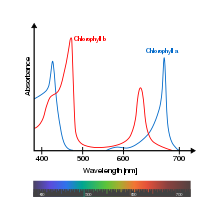
\includegraphics[width=0.4\textwidth]{wavelength.png}
	\caption{PBR Material}
	\label{clorophyll}
\end{figure}

\subsubsection{Specularity}
Every plant has its own manner of protection. One of these manners is having special layers on the leaves. The outer layer is usually covered with different materials like cutin and natural wax which mostly contain  alcohol, alkaline and fatty acid. The Wax the wax itself provides a certain specularity of the leaf. This specularity needs to be simulated, because there might appear some specularity effects which might change the appearance of an object that usually has a fix color. For example if light falls directly on the leaf there might appear a bright white spot. This will later on not be seen as a leaf in the total leaf area that is mesaured, because the color differs from the green that is detected.

\subsubsection{Roughness}
The stucture of the leaves might have an impact on the viewable color aswell. A leaf as we know it, is not a 2d surface, but more a three dimensional object with a certain structure. A leaf contains three major aspects that let it appear in a more threedimensional way. The first two are the leaf stem and the veins forking from it. The thrid is the microstructural setting.

\subsection{Color- and Materialchange in Blender}
\input{members/kh/authors}

In this part we will look at the color and material change inside of Blender. As described in the section before, the plants from Plant-Studio have already been inserted and have the correct positioning. We decided to insert 10 plant randomly chosen from the 42 plants we generated before. The generated plants have a big number of leaves and fruits so we can reduce them afterwards, to have a more variant simulation. \newline
All plants together have a mean of 211 leaves and 101 fruits.
To get a more realistic and reliable model of the plants we change the color and the material of the plants. This is necessary because the leaf area algorithm needs reliable data to work with. It's easy to understand, that an object can differ in the appearence when the light falls on it from different angles. Therefore we need material properties that are similar to the properties of of real leafs and fruits.
Blender gives many options to change the properties of a material. In the following we will discuss the properties: color(appearence), metallic, emission, roughness , reflectiveness and normals. These facets are part of the pbr-library in Blender(Figure \ref{pbr}).
The changes made in this section will mainly focus on the topside of the leaf(the side that faces the sun). This is based on the fact, that the leafarea is calculated by taking a snapshot from the top of the plant. The bottom-side will be irrelevant and will be neglected in the simulation.

\subsubsection{Blender properties}
\begin{figure}[h]
	\centering
	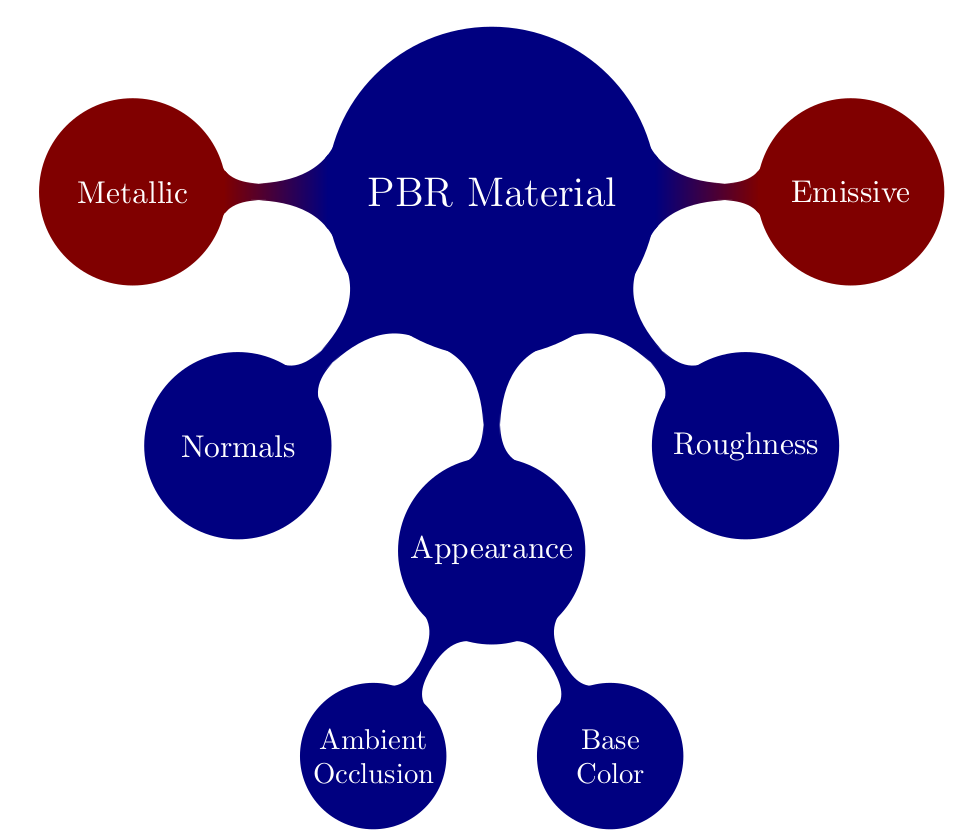
\includegraphics[width=0.6\textwidth]{blender_properties.png}
	\caption{PBR Material}
	\label{pbr}
\end{figure}
\textbf{Appearence}\\
This property can be splitted in two components. The color and the ambient occlusion. The color modifies the RGB-Values of an Object. The ambient occlusion simulates shadows between different objects, even if there is no light source in the scenery. In the simulation of the leaves and the tomatoes, the focus will mainly be on the color.\\


\textbf{Roughness}\\
The roughness is a property that is realized by a gray scale. The micro-surface of the material changes to a slightly rougher structure and this changes the looks and reflectionproperties when it comes to shading and rendering. \newline

\textbf{Metallic}\\
The option metallic is a binary map that specifies the metallic properties of a material. It is either metallic or dielectrit. It is made visible by a certain absorbtion of a material.\\


\textbf{Emission} \\
The emission describes the light a material will emit. So the material itself will become a light source and may shine. This is often used to give the scenery different illuminations. It is realized by a gray scale map that specifies the light radiation of a material, mostly to show heat or illumination.\\


\textbf{Normals} \\
A normal describes the direction an object points to. It is usually an orthogonal vector on a surface which leads to the side which shall be visible to the camera. It is important for shading, lighting  and the visibility of the surface itself.\\

\subsection{Materialchange: practical approach}
\%input{members/kh/authors}
Since the leaves are already imported into blender, it is only necessary to take certain objects and color these in another color. As described before this task is approached by adding a new material to an object. In the following paragraphs the Pythoncode will be described. \newline
Coloring the leaves is performed in three steps.


\subsubsection{Selecting Objects}
To select objects in blender a scenery has to be picked first. The scenery contains the objects that need to be edited later on. The leaves are easiely picked by looping over all elements inside the scenery. All Elements with the suffix ''Leaf'' are added to an array so they can be accessed later.
\lstset{language=Python, frame=single}
\begin{lstlisting}
# defining scenery
scene = bpy.context.scene


# fetching Leaves
leafs = [obj for obj in scene.objects
if fnmatch.fnmatchcase(obj.name, "*Leaf")]
\end{lstlisting}

\subsubsection{Creating Material}
Since all leaves have been detected, a new material needs to be established. As described in the previous section the color, metallic, specularity and roughness of the material will be edited, so the leaf gets the structure as described.
\lstset{language=Python, frame=single}
\begin{lstlisting}
# defining a new material with name "brown"
mat_brown = bpy.data.materials.new("brown")


# setting the Properties of the material
mat_brown.diffuse_color = (0.091, 0.014, 0, 8)
mat_brown.metallic = (0.65)
mat_brown.specular_intensity = (0.5)
mat_brown.roughness = (0.55)
\end{lstlisting}

\subsubsection{Applying Material}
To apply the material to the leaves the existing material needs to be deleted first, otherwise Blender would not set the new material as a first priority to the object. After this the material can be applied to the object. This will be performed in a loop over all elements inside the array with all leaves.

\lstset{language=Python, frame=single}
\begin{lstlisting}
#getting number of leaves
leafs_count = len(leafs)

for i in range(0, leafs_count, 1):
mesh = leafs[i]

#deleting all existing meterials
mesh.data.materials.clear()

#applying new material
mesh.data.materials.append(mat_brown)
\end{lstlisting}


\begin{figure}[h]
\centering
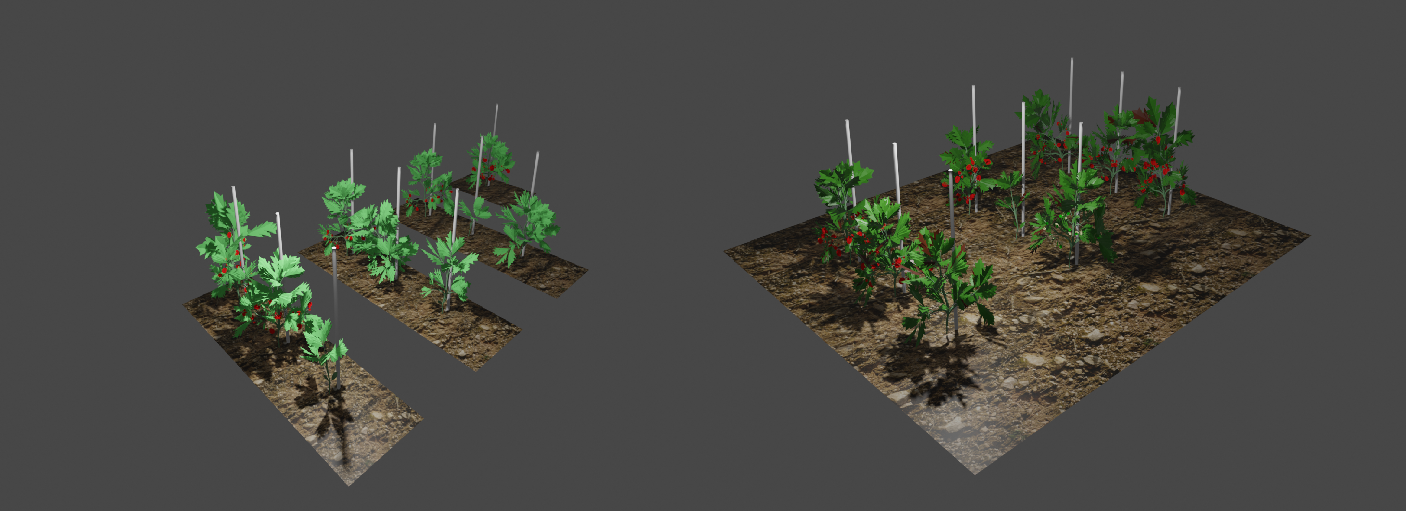
\includegraphics[width=1\textwidth]{coloring.png}
\caption{Coloring}
\label{coloring}
\end{figure}


\subsection{Removing Objects}
\input{members/kh/authors}

To approach a high variability the pregenerated plants also need to have the number of leaves and fruits reduced.
In the following it is described how the practical Aspect of removing leaves and fruits is done in Blender.
As an example it is shown how all leaves on a plant are deleted. \newline
First all leaves need to be detected and stored inside of an array. Then every element of the Array is accessed and deleted from the scenery.
\lstset{language=Python, frame=single}
\begin{lstlisting}
#fetching all leaves
leafs = [obj for obj in col.objects
if fnmatch.fnmatchcase(obj.name, "*Leaf*")]

#delete all objects inside of the Array
bpy.ops.object.delete({"selected_objects": leafs})
\end{lstlisting}
To get the same result for the fruits, the keyword ''fruit'' with wildcards surrounded needs to be accessed while fetching. A fruit in the case of the pregenerated tomatoplant is compounded by ten fruit elements to get a circular structure. To delete a whole fruit it is necessary to delete ten fruit elements. Since all elements of a fruit lay right next to each other inside the array it is easy to just loop over all fruits and delete always ten elements at a time to remove a whole fruit.
\newline
The removal of objects is shown in Figure \ref{order}.

\begin{figure}[h]
\centering
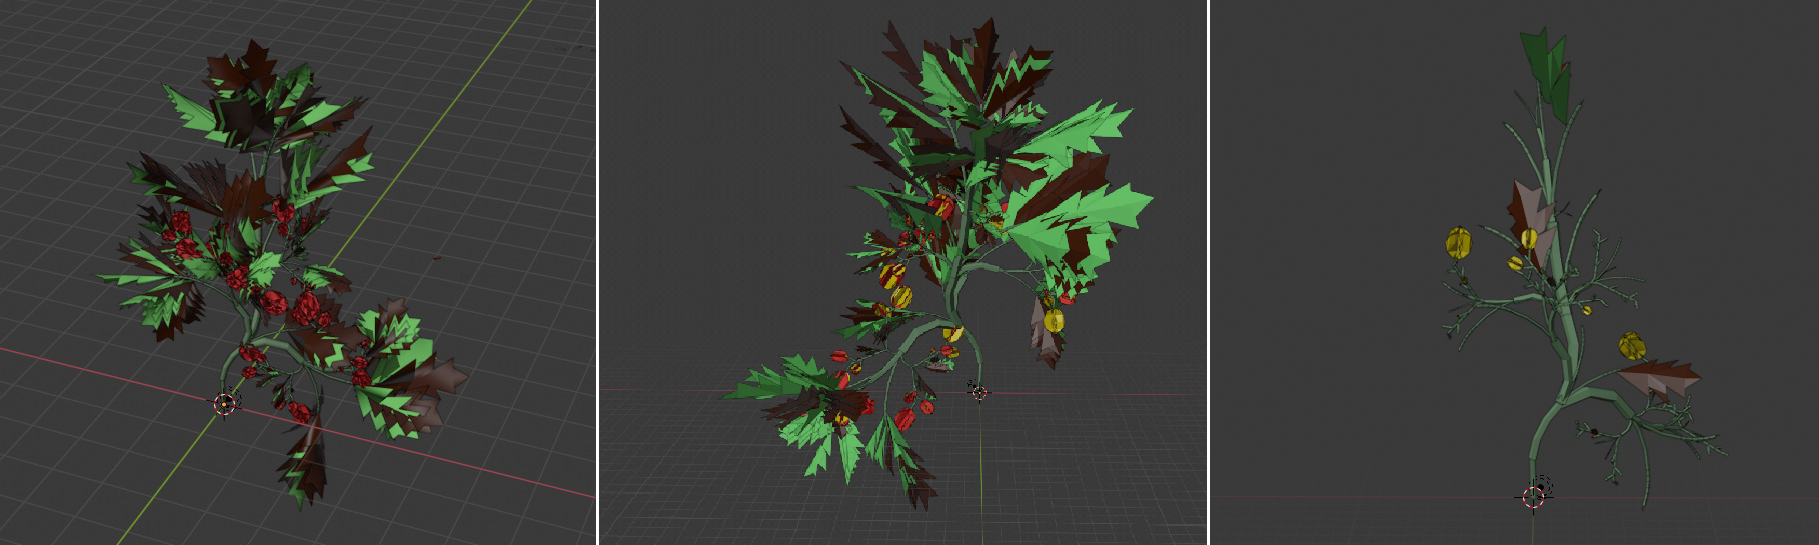
\includegraphics[width=1\textwidth]{examples.png}
\caption{Objectremoval}
\label{order}
\end{figure}


\subsection{Textures in Blender}
\input{members/kh/authors}
The following section is just a small outlook. The practical implementation like applying textures or chosing the correct tools in Blender will no be discussed on this point.\newline
As already mensioned before the system needs reliable data to work with, so it is the task of the simulation to get the plants to look as realistic as possible. Real leaves have spots that reflect the light and shading that lets the collor appear differently. To apply these settings it will be necessarry to work with a texture based approach to get the leaves look better in future simulation. 
To get these textures we basically need a picture or an already existing texture. There are a few requires Stepts to apply a texture to an object in Blender, so all gaps, shades, lightings, reflections and bumps are as realistic as possible.
Overall there are a few textures needed wich can all be excluded from an already existing picture.
In the following paragraphs the textures are described an can be seen in figure \ref{textures} :
\subsubsection{Diffuse Texture}
The diffuse texture is the original bitmap. This picture is the root where all the followig textures are generated from. This picture has to contain all information that should be added to the object inside of Blener.
\subsubsection{Normal Texture}
The normal texture is a bumpmap. It shows small bumps and roughnesses in the structure of the object. It adds more detail to the shading, without increasing the number of polygons the object is made of. 
\subsubsection{Specularity Texture}
The specularity texture tells the program which part of the object are glossy and which are black. The object can be reflective like metal, ceramic or plastic. It is usually a greyscale map where the black and white parts of the map highlight specularity of a pixel.
\subsubsection{Occlusion Texture}
The occlusionmap adds more detail to the object. Is stores information about depth and shadows inside of an object. May Objects already have a more rough structure and more depth than a picture printed on an object can show.
\subsubsection{Displacement Texture}
The displacementtexture stores the 3D information of an image. A surface is usually not 2D and in the case of a leaf it is certain that it has a structure defined my the stam and the veins goin out of it as describes by the modeler. To have these parts stick out more, the displacementmap adds the 3D details to an object.
\begin{figure}[h]
	\centering
	\includegraphics[width=1\textwidth]{textures.png}
	\caption{Diffuse/Normal/Specularity/Occlusion/Displacement}
	\label{textures}
\end{figure}

\newpage

\clearpage
\section{Implementation}\label{sec:implementation-and-evaluation}
\input{members/ssr/authors}

Within the given time constraints of the project the entire design couldn't be implemented, evaluated and refined.
Nonetheless, an implementation has been conducted to test the pipelines and evaluate the practicality of the modelling ideas
and to gather data, such as:

\begin{enumerate}
    \item Segmenting leaf area from non-leaf area to estimate the leaf area visible from above - for the LAI computation
    \item Gathering color distributions of leaf areas, based on the segmentation.
    \item Locating the tip of the plant - for the height estimation
\end{enumerate}

A general description of the pipeline and high-level ideas have been describe in the model section, this
section however exactly explains how the mentioned aspects have been extracted which are the main metrics for
further computations.\\

Firstly, the general architecture and platform are briefly described and then each step of the computational
pipeline with example outputs are shown.
\graphicspath{{members/ssr/figures/}}

\subsection{Pipeline and Algorithms}\label{subsec:pipeline}

This section provides a detailed look at the implementation level of the selected algorithms
with all its parameters.

\subsubsection{Pipeline A}

Since the greenhouse domain provides an highly constrained environment and setup the two main tasks
of canopy segmentation and plant tip location can be solved for very specific cases.

Firstly, it is assumed that only \textit{one} plant canopy per image is visible due to the way the
crop and camera is arranged in the greenhouse - since this is a requirement for the system.

As described in the \ref{subsec:segmentation} this allows a simple segmentation which works well -
as shown in figure \ref{fig:seg:1}, \ref{fig:seg:2}, \ref{fig:seg:3}, \ref{fig:seg:4}.

\begin{figure}[H]
    \centering
    \begin{minipage}[b]{0.24\textwidth}
        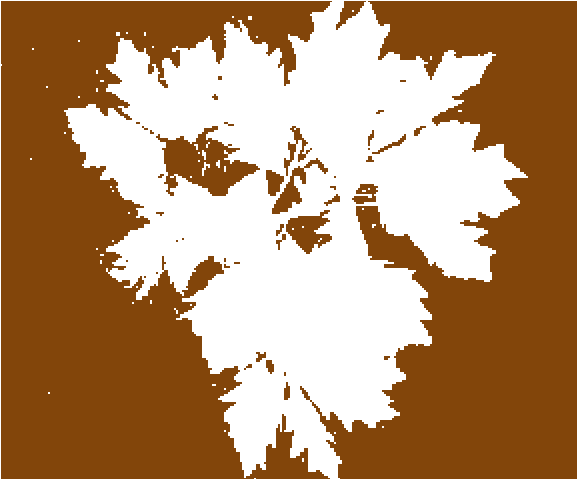
\includegraphics[width=\textwidth]{implementation/segment-1.png}
        \caption{Cluster non-leaf}
        \label{fig:seg:1}
    \end{minipage}
    \hfill
    \begin{minipage}[b]{0.24\textwidth}
        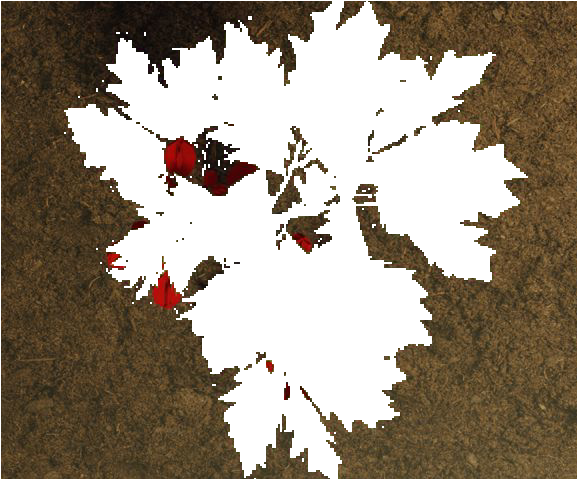
\includegraphics[width=\textwidth]{implementation/segment-2.png}
        \caption{Non-leaf texture}
        \label{fig:seg:2}
    \end{minipage}
    \hfill
    \begin{minipage}[b]{0.24\textwidth}
        \frame{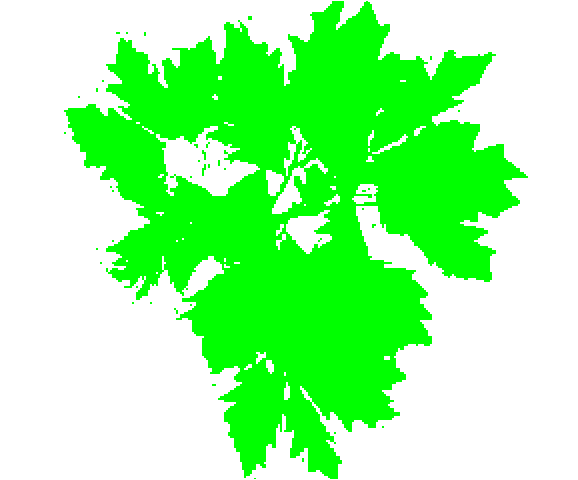
\includegraphics[width=\textwidth]{implementation/segment-3.png}}
        \caption{Cluster leaf}
        \label{fig:seg:3}
    \end{minipage}
    \hfill
    \begin{minipage}[b]{0.24\textwidth}
        \frame{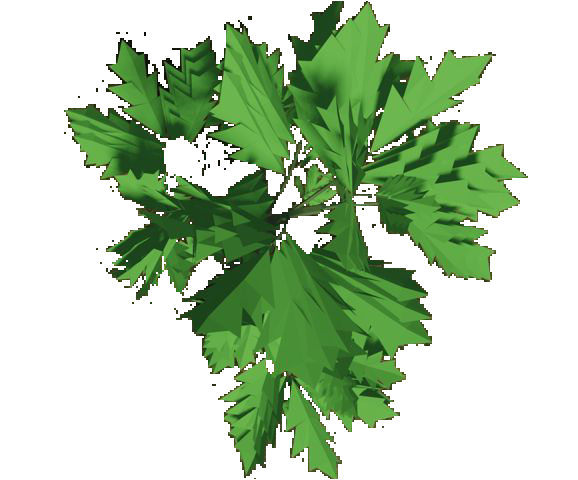
\includegraphics[width=\textwidth]{implementation/segment-4.png}}
        \caption{Texture leaf}
        \label{fig:seg:4}
    \end{minipage}
\end{figure}
\subsubsection{Pipeline B}

Pipeline B is concerned with finding the tip of the plant.
This is achieved by finding the highest point along the plant's stake which is covered by leaves.

For this purpose the longest vertical edge within an image is detected and it's lower point is
expected to be the plant's tip.

The following algorithm (or computational pipeline) has been developed in order to achieve this goal,
followed by a more formal description of the algorithm.

\begin{enumerate}
    \setlength{\itemsep}{0pt}
    \setlength{\parskip}{0pt}
    \item Edge detection to find contours
    \item Vertical blur to combine interrupted vertical lines (due to edge filter)
    \item High pass filter to create binary image of lines, this eliminates dots and short lines
    \item Count vertical line column-wise. Allow a horizontal tolerance window to accept slight slopes
    \item The lower point of the longest line is assumed to be plants stake
\end{enumerate}

The exact chosen algorithms have been gradually developed and refined by experimenting
based on images generated from the simulation or actual images from tomato plants.\\

\textbf{Edge detection:} There are plenty of edge detection algorithms to choose from but since
the final goal here only to locate vertical edges a simple and edge filter is sufficient, especially
it must must not find contours but find edges across color variations.

For this purpose the \textit{Sobel operator} has been chosen which is efficient and sufficient
for this purpose and combined with a high pass filter.
It uses two 3x3 kernels which are convoluted on the input image $I$ to approximate the horizontal
and vertical derivative at each pixel.\\

\noindent\begin{minipage}{.5\linewidth}
     \begin{equation}
         G_{x} = \begin{bmatrix}
                     +1 & 0 & -1\\
                     +2 & 0 & -2\\
                     +1 & 0 & -1
         \end{bmatrix} \ast I
     \end{equation}
\end{minipage}
\begin{minipage}{.5\linewidth}
    \begin{equation}
    G_{y} = \begin{bmatrix}
                +1 & +2 & +1\\
                0 &  0 &  0\\
                -1 & -2 & -1
    \end{bmatrix} \ast I
    \end{equation}
\end{minipage}\\

Which result in the x-coordinate as the increasing \textit{right} direction and y-coordinate as
increasing \textit{down} direction.
The gradient magnitude and direction can be calculated as follows:

\noindent\begin{minipage}{.5\linewidth}
             \begin{equation}
                 G = \sqrt{G_{x}^{2} + G_{y}^{2}}
             \end{equation}
\end{minipage}
\begin{minipage}{.5\linewidth}
    \begin{equation}
        \Theta = atan\left(\frac{G_{y}}{G_{x}}\right)
    \end{equation}
\end{minipage}\\

These values are in the implementation combined with a range check and low pass filter to better results:

\lstinputlisting[language={[Sharp]C}, caption = Edge dectection]{members/ssr/code/edge.cs}\vspace{5pt}

\textbf{Vertical Blur:} This applies just repeatedly a vertical average blur:
\begin{equation}
    \frac{1}{3}\begin{bmatrix}
        1 & 1 & 1
    \end{bmatrix}^{T}
\end{equation}

\textbf{High pass:} Only grey values below a certain threshold, which leads to removal of irrelevant
smaller dots and lines, see figure \ref{fig:v:3}\\

\textbf{Finding longest vertical edge:} At this point only a binary black and white image has remained.
Finding the longest vertical edge is conducted by preparing a boolean matrix in multiple steps.
Firstly, for every pixel a horizontal interpolation of adjacent horizontal pixels, along a variable
window is applied. This allows to include lines with a slight slope.

\lstinputlisting[language={[Sharp]C}, caption = Interpolate each pixel horizontally]{members/ssr/code/hinterpolate.cs}\vspace{5pt}

Now a boolean matrix has been constructed which is column-wise traversed to the longest sequence of true
values (longest vertical interpolated line):

\lstinputlisting[language={[Sharp]C}, caption = Find longest vertical boolean sequence]{members/ssr/code/vline.cs}\vspace{5pt}

The following figure shows the result of each step with the final results.

\begin{figure}[H]
    \centering
    \begin{minipage}[t]{0.24\textwidth}
        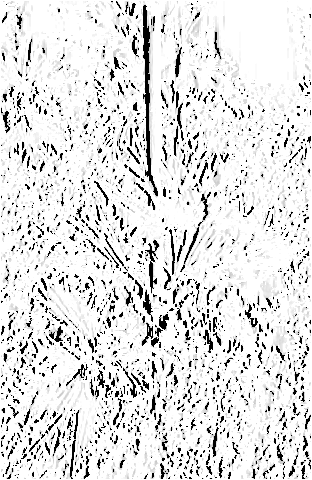
\includegraphics[width=\textwidth]{implementation/v-1.png}
        \caption{Sobel operator}
        \label{fig:v:1}
    \end{minipage}
    \hfill
    \begin{minipage}[t]{0.24\textwidth}
        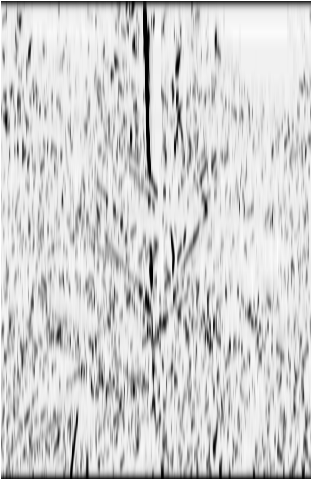
\includegraphics[width=\textwidth]{implementation/v-2.png}
        \caption{Vertical blur}
        \label{fig:v:2}
    \end{minipage}
    \hfill
    \begin{minipage}[t]{0.24\textwidth}
        \frame{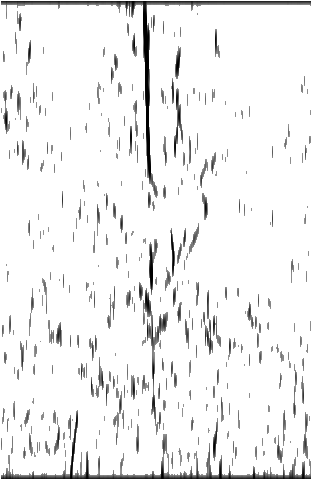
\includegraphics[width=\textwidth]{implementation/v-3.png}}
        \caption{High pass}
        \label{fig:v:3}
    \end{minipage}
    \hfill
    \begin{minipage}[t]{0.24\textwidth}
        \frame{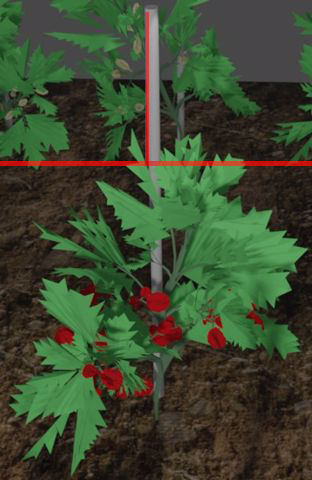
\includegraphics[width=\textwidth]{implementation/v-4.png}}
        \caption{Detection plant tip}
        \label{fig:v:4}
    \end{minipage}
\end{figure}
\input{members/ssr/implementation/pipeline-overview.tex}
\subsection{Architecture and Platform}\label{sec:architecture}

The architecture of the system are based on multiple individual components which have been implemented
independently consisting on following parts:

\begin{enumerate}
    \item Core API for image processing (computational pipeline) \cite{greenhouseplusplus}
    \item Web API making the core API accessible from network \cite{greenhouseplusplus}
    \item Desktop client in Visual C\# 2019 \cite{greenhouseplusplus}
    \item Web based progressive web app (PWA) allowing network access of the pipeline \cite{greenhouseplusplus:app}
\end{enumerate}

Figure \ref{fig:arch} shows the high level architecture of the entire application ecosystems.

\begin{figure}[H]
    \centering
    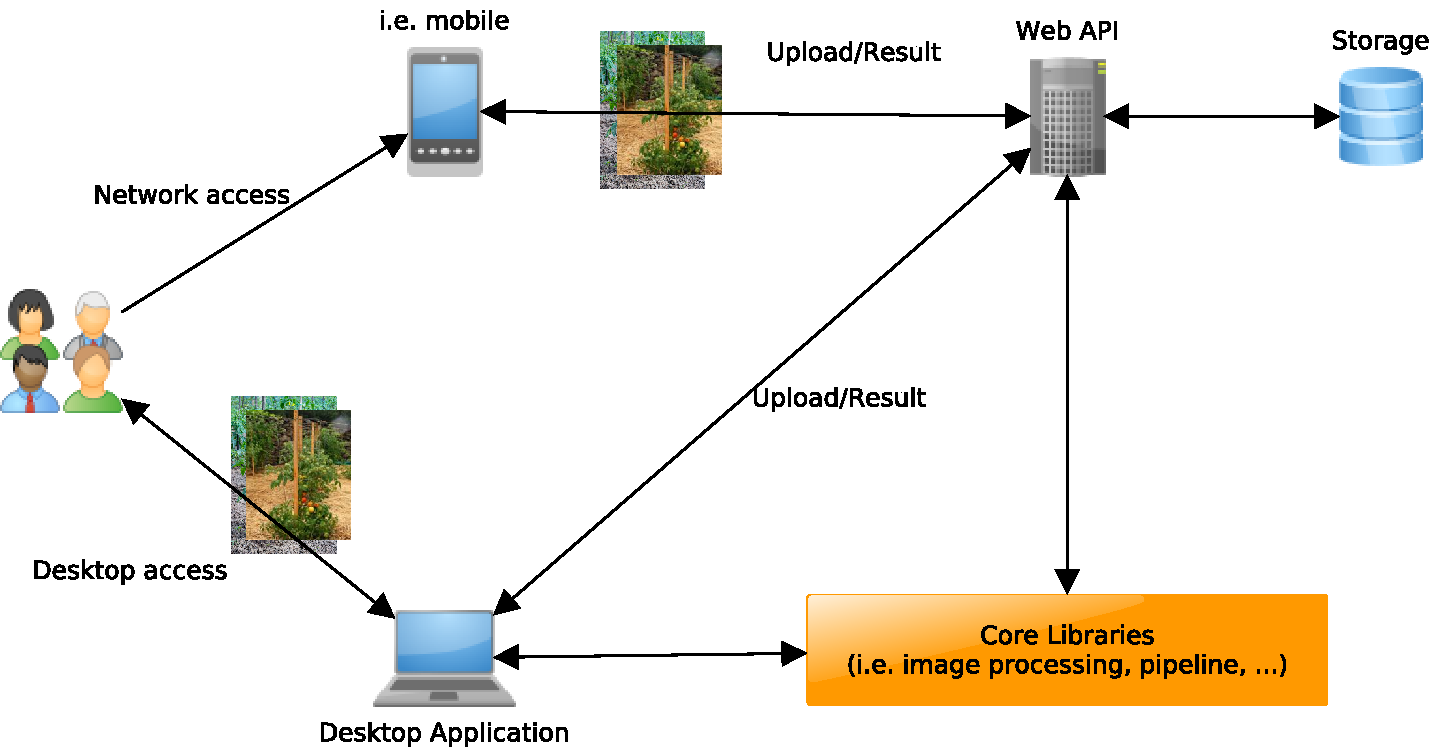
\includegraphics[width=1.0\textwidth]{implementation/architecture.pdf}
    \caption{The pipeline can be accessed by web browser or purely on a Windows desktop.}
    \label{fig:arch}
\end{figure}

The purpose of this architecture is - beside clean implementation and testability - to test a flexible
solution which might also be deployed and used under varying conditions, locations and limited resources.
Figure \ref{fig:desktopclient} and \ref{fig:webclient} show the desktop and web clients
which conduct the plant tip location and segmentation.\\

The implementation of this project is freely accessible and open-source on Github
at \cite{greenhouseplusplus} and \cite{greenhouseplusplus:app} and the web interface is accessible
on a test-server at \cite{greenhouseplusplus:live}.

\begin{figure}[H]
    \centering
    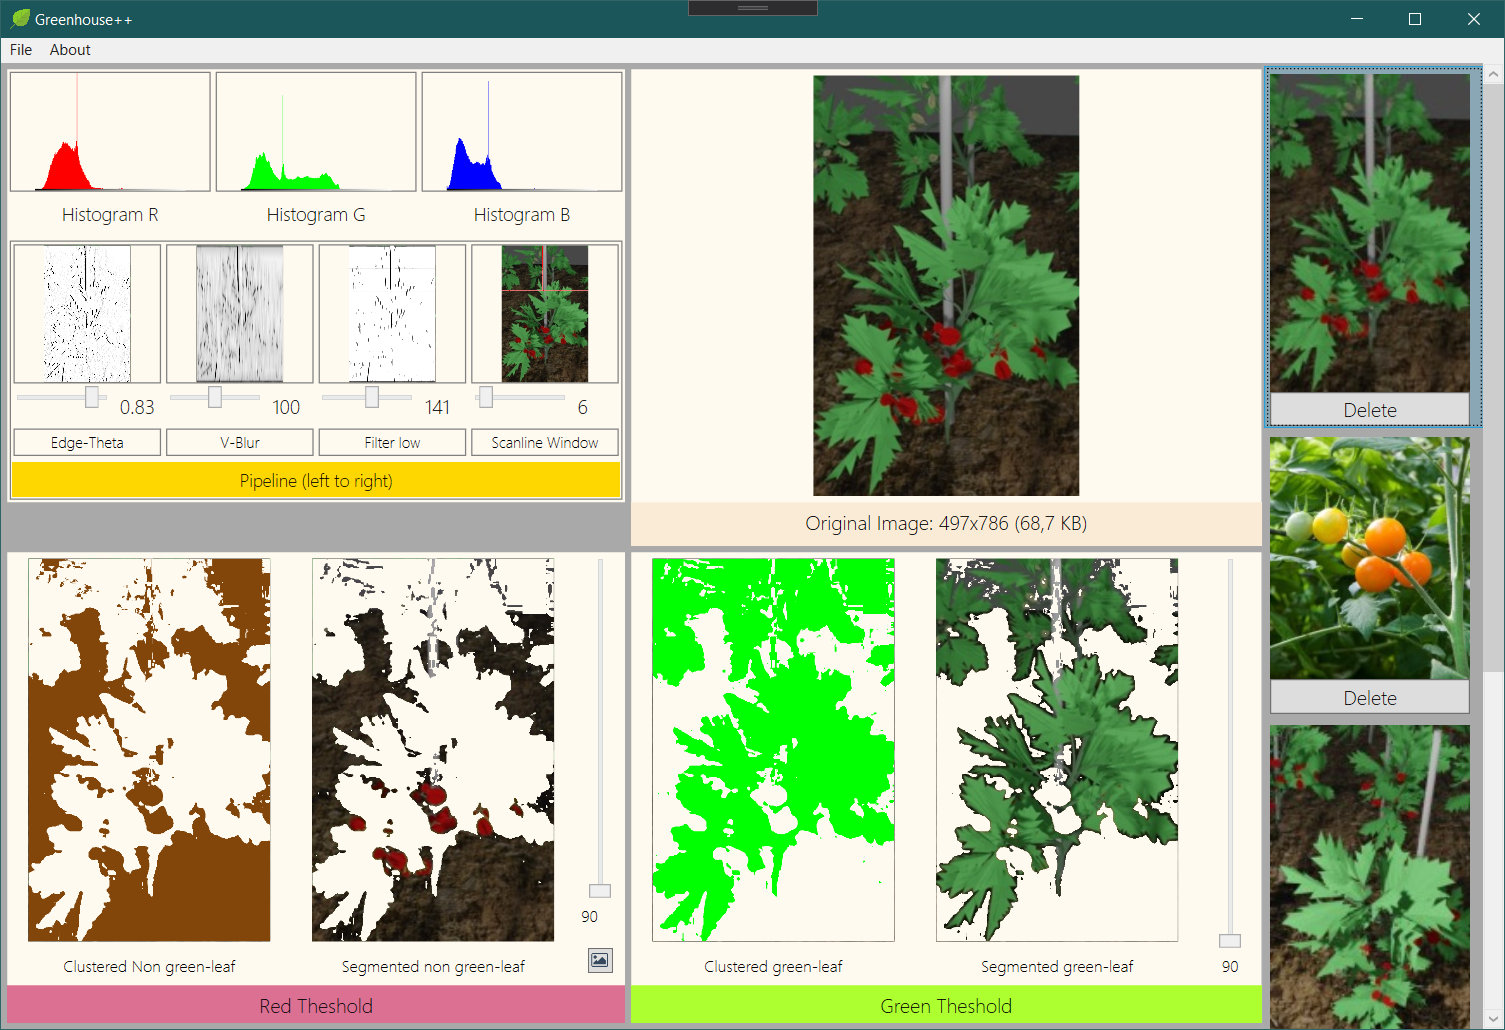
\includegraphics[width=0.9\textwidth]{implementation/greenhouseplusplus-ui.jpg}
    \caption{Visual C\# 2019 Desktop client}
    \label{fig:desktopclient}
\end{figure}

\begin{figure}[H]
    \centering
    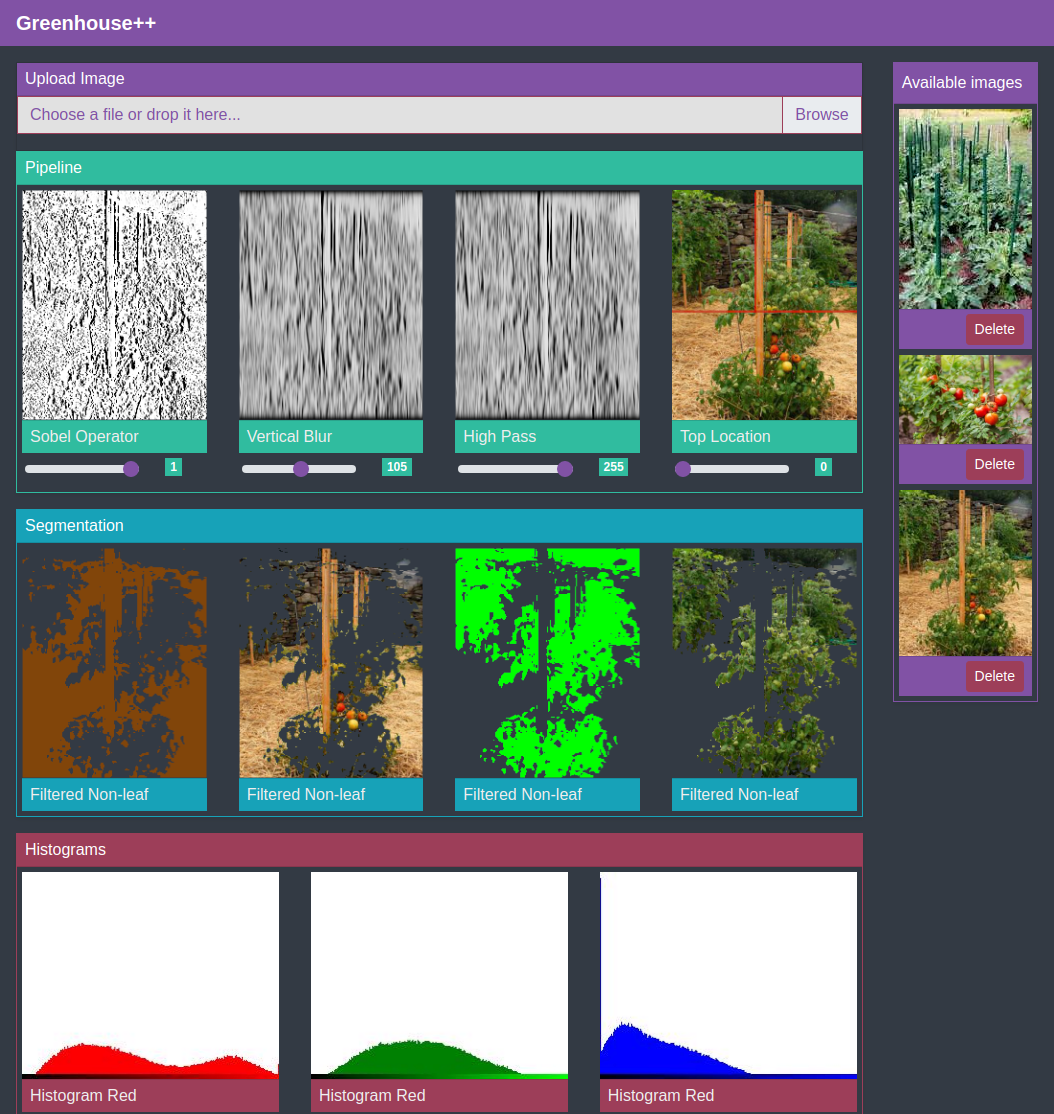
\includegraphics[width=0.6\textwidth]{implementation/web-ui.png}
    \caption{Web based client}
    \label{fig:webclient}
\end{figure}
%\subsection{Implementation}\label{subsec:implementation}

\begin{figure}[h!]
    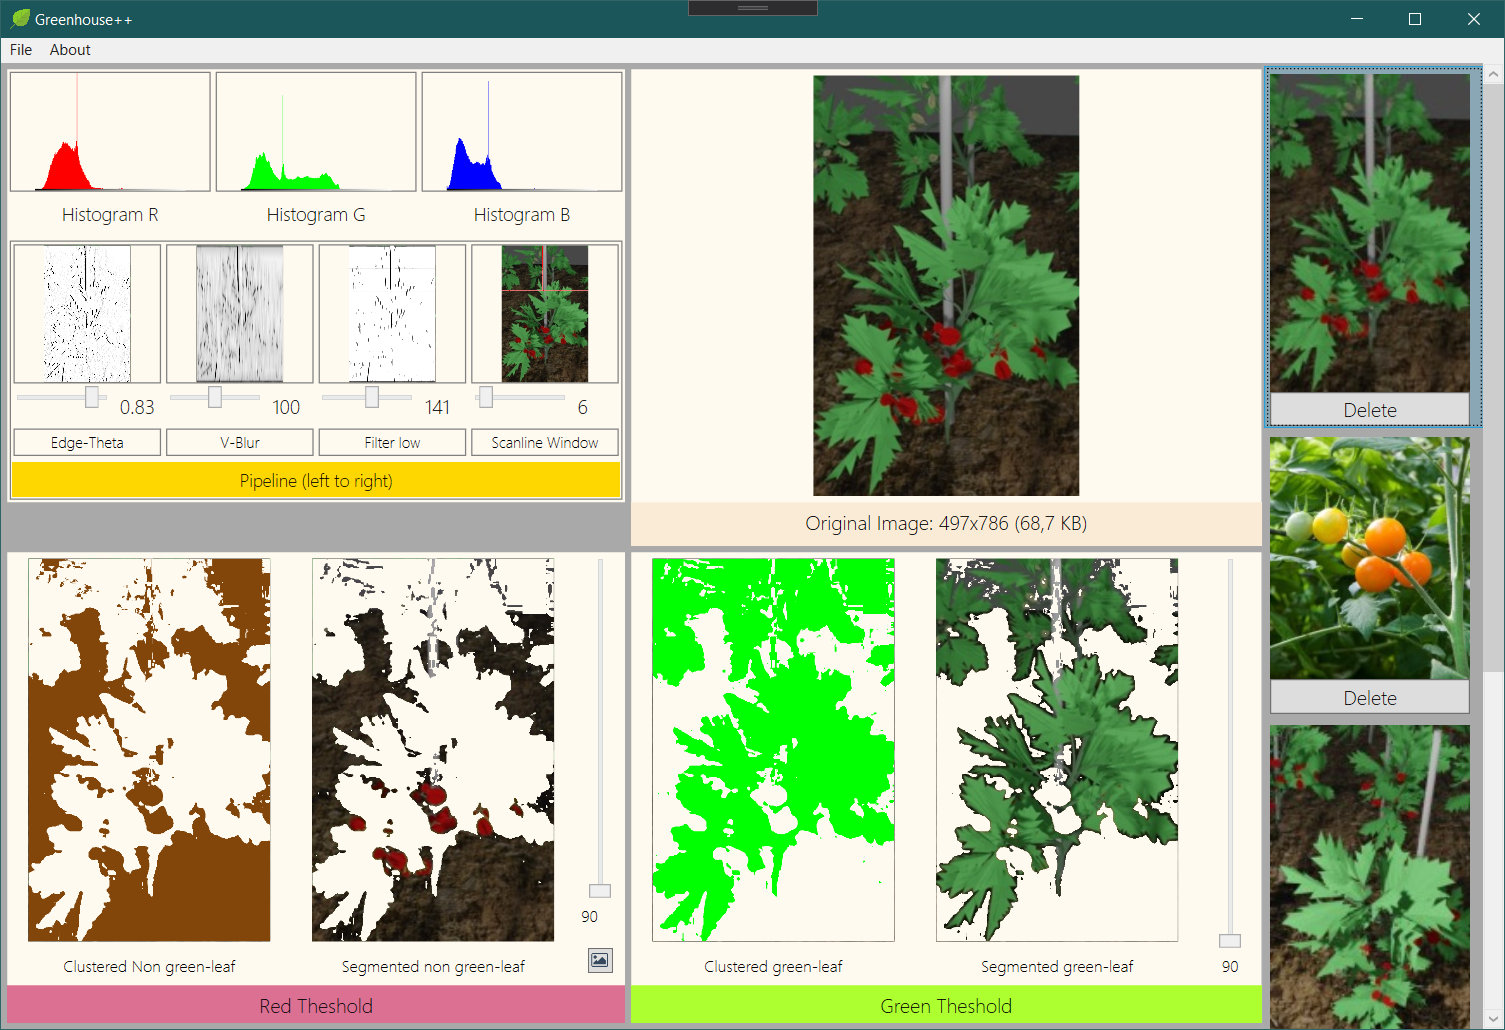
\includegraphics[width=\textwidth,height=\textheight,keepaspectratio]{implementation/greenhouseplusplus-ui.jpg}
    \caption{Greenhouse++ User Interface}
    \label{greenhouseplusplus:ui}
\end{figure}
%\subsection{Evaluation}\label{subsec:evaluation}

..
%\input{sections/discussion}
\section{Conclusion}\label{sec:conclusion}

Todo
\section{Outlook}\label{sec:outlook}

This prokect is meant to be continued and improved in another class. Future work will include finding starting values for training parameters, testing the whole pipeline with simulated picture followed by an analization of its performance, training of parameters and
adjustments of model and pipeline. The performance of the single tasks will reveal the quality of the choosen methods and models. Those might be adjusted or replaced. A description of the future yield development could also be included in the model, since it is an important part but only poorly modelled jet.


\newpage
\printbibliography

\end{document}
